\documentclass[12pt,letterpaper,oneside]{report}

% -----------------------------------------------------------------------
% IDIOMA Y CODIFICACIÓN
% -----------------------------------------------------------------------
\usepackage[utf8]{inputenc}
\usepackage[T1]{fontenc}
\usepackage[spanish,es-tabla,es-nodecimaldot]{babel}
\usepackage{csquotes}

% -----------------------------------------------------------------------
% TIPOGRAFÍA (Times-like) Y MICROTIPOGRAFÍA
% -----------------------------------------------------------------------
\usepackage{mathptmx} % Times (texto + matemáticas)
\usepackage{microtype} % mejor justificación y cortes de palabra

% -----------------------------------------------------------------------
% ESPACIADO (IPN: 1.5) + PÁRRAFOS
% -----------------------------------------------------------------------
\usepackage{setspace}
\onehalfspacing

% Sangría estándar y separación controlada (no cambia tu contenido)
\setlength{\parindent}{1.25cm}
\setlength{\parskip}{0pt}

% -----------------------------------------------------------------------
% MÁRGENES (encuadernación) Y HEADER/FOOTER
% -----------------------------------------------------------------------
\usepackage{geometry}
\geometry{
  letterpaper,
  left=3.5cm,
  right=2.5cm,
  top=2.5cm,
  bottom=2.5cm,
  headheight=14.5pt,
  headsep=0.7cm,
  footskip=1.2cm
}

% -----------------------------------------------------------------------
% PAQUETES MATEMÁTICOS
% -----------------------------------------------------------------------
\usepackage{amsmath}
\usepackage{amsfonts}
\usepackage{amssymb}

% -----------------------------------------------------------------------
% ALGORITMOS Y PSEUDOCÓDIGO
% -----------------------------------------------------------------------
\usepackage{algorithm}
\usepackage{algpseudocode}
\floatname{algorithm}{Algoritmo}
\renewcommand{\listalgorithmname}{Lista de Algoritmos}
\algrenewcommand\algorithmicrequire{\textbf{Entrada:}}
\algrenewcommand\algorithmicensure{\textbf{Salida:}}

% -----------------------------------------------------------------------
% DISEÑO, IMÁGENES Y TABLAS
% -----------------------------------------------------------------------
\usepackage{graphicx}
\usepackage{xcolor}
\usepackage{tikz}
\usetikzlibrary{calc, shapes, arrows, positioning, automata, bending, arrows.meta, babel}
\usepackage{enumitem}
\usepackage{float}
\usepackage{caption}
\usepackage{subcaption}
\usepackage{array}
\usepackage{booktabs} % tablas más formales (no afecta si no lo usas)
\usepackage{pdflscape} % Permite rotar hojas individuales en el PDF
\usepackage{svg}
\usepackage{pgfplots}
\usepackage{tabularx}
\usepackage{xltabular}
\usepackage{colortbl}
\usepackage{worldflags}
\flagsdefault[width=0.45cm]

% Listas más limpias (sin tocar texto: solo formato)
\setlist[itemize]{noitemsep, topsep=3pt}
\setlist[enumerate]{noitemsep, topsep=3pt}

% Colores (portada)
\definecolor{guinda}{RGB}{108, 19, 43}
\definecolor{esimegreen}{RGB}{0, 103, 56}
\definecolor{rowgray}{HTML}{F8F9FA}

% Figuras y tablas
\captionsetup[figure]{labelfont={bf}, name={Figura}, labelsep=period}
\captionsetup[table]{labelfont={bf}, name={Tabla}, labelsep=period}

% -----------------------------------------------------------------------
% CONTROL DE VIUDAS/HUÉRFANAS (estándar tesis/tesina)
% -----------------------------------------------------------------------
\clubpenalty=10000      % evita viudas (primera línea sola)
\widowpenalty=10000     % evita huérfanas (última línea sola)
\displaywidowpenalty=10000

% -----------------------------------------------------------------------
% HIPERVÍNCULOS (PDF) - compatible con biblatex
% -----------------------------------------------------------------------
\usepackage[hidelinks]{hyperref}
\hypersetup{
  colorlinks=true,
  linkcolor=black,
  citecolor=black,
  urlcolor=blue,
  pdftitle={Tesina},
  pdfauthor={Antonio Torres}
}

% -----------------------------------------------------------------------
% BIBLIOGRAFÍA [IEEE] CON BIBLATEX (mantienes biber)
% -----------------------------------------------------------------------
\usepackage[backend=biber,style=ieee]{biblatex}
\addbibresource{./lib/referencias.bib}

% -----------------------------------------------------------------------
% ENCABEZADOS Y PIES (formato de tesina: limpio y formal)
% -----------------------------------------------------------------------
\usepackage{fancyhdr}
\pagestyle{fancy}
\fancyhf{} % limpia todo
\fancyfoot[C]{\thepage} % número al centro abajo (común en tesinas)
\renewcommand{\headrulewidth}{0pt}
\renewcommand{\footrulewidth}{0pt}

% -----------------------------------------------------------------------
% FORMATO DE TÍTULOS DE CAPÍTULO (sin invadir márgenes)
% -----------------------------------------------------------------------
\usepackage{titlesec}
\titleformat{\chapter}[display]
  {\normalfont\huge\bfseries}{\chaptertitlename\ \thechapter}{18pt}{\Huge}
\titlespacing*{\chapter}{0pt}{-10pt}{30pt}

% -----------------------------------------------------------------------
% DATOS DEL DOCUMENTO
% -----------------------------------------------------------------------
\title{Ecosistema multiagente basado en LLM y aprendizaje por refuerzo para la generación y validación de circuitos analógicos CA/CD a partir de lenguaje natural}
\author{Antonio Torres}
\date{\today}

\begin{document}

  % ---------------------------------------------------------------------
  % PRELIMINARES
  % ---------------------------------------------------------------------
  \pagenumbering{roman}

  % 1. PORTADA
  % Contenido de la portada
\begin{titlepage}
    \begin{tikzpicture}[remember picture, overlay]
    
        \coordinate (topleft) at ($(current page.north west) + (2.5cm, -2cm)$);
        \coordinate (bottomleft) at ($(current page.south west) + (2.5cm, 2.5cm)$);
        
        % 1. LOGO IPN (Arriba Izquierda)
        \node[anchor=north, inner sep=0pt] at (topleft) {
            
\includegraphics[width=4cm]{../src/logos/ipn_logo.png}
        };
        
        % 2. LOGO ESIME (Abajo Izquierda)
        \node[anchor=south, inner sep=0pt] at (bottomleft) {
            
\includegraphics[width=3cm]{../src/logos/esime_logo.jpg}
        };
        
        % 3. LÍNEAS VERTICALES LATERALES
        % Línea gruesa
        \draw[esimegreen, line width=2pt] 
            ($(topleft) + (0, -3.2cm)$) -- ($(bottomleft) + (0, 3.8cm)$);
        % Línea delgada paralela
        \draw[esimegreen, line width=1pt] 
            ($(topleft) + (0.15cm, -3.2cm)$) -- ($(bottomleft) + (0.15cm, 3.8cm)$);
            
        % 4. ENCABEZADO SUPERIOR
        \node[anchor=north] at ($(current page.north) + (1cm, -2.5cm)$) {
            \begin{minipage}{14cm}
                \centering
                \large\textbf{INSTITUTO POLITÉCNICO NACIONAL}\\[0.4cm]
                
                % Líneas horizontales verdes
                {\color{esimegreen}\hrule height 2pt}
                \vspace{0.1cm}
                {\color{esimegreen}\hrule height 1pt}
                \vspace{0.4cm}
                
                \large\textbf{ESCUELA SUPERIOR DE INGENIERÍA MECÁNICA Y ELÉCTRICA}\\
                \textbf{UNIDAD CULHUACÁN}
            \end{minipage}
        };
    \end{tikzpicture}

    % --- CONTENIDO DE TEXTO CENTRAL ---
    \vspace*{5cm} 
    \centering
    
    {\LARGE \textbf{TESINA}}\\[0.8cm]
    
    {\Large \textit{Ecosistema multiagente basado en LLM y aprendizaje por refuerzo para la generación y validación de circuitos analógicos CA/CD a partir de lenguaje natural}}\\[1.5cm]
    
    \large QUE PARA OBTENER EL TÍTULO DE:\\[0.3cm]
    \textbf{INGENIERO EN COMPUTACIÓN}\\[1.5cm] 
    
    \large PRESENTA:\\[0.3cm]
    \textbf{ANTONIO DE JESUS TORRES MARTÍNEZ}\\[0.3cm]
     \textbf{DIEGO JESUS GUTIERREZ DELGADO}\\[1.5cm]
    
    \large ASESOR:\\[0.3cm]
    \textbf{RICARDO ISRAEL CALZADA SALAS}\\[1.5cm]

    \vfill
    
    \normalsize Ciudad de México \today
    
\end{titlepage}
  \clearpage

  % 2. RESUMEN Y ABSTRACT
%   \input{sections/resumen}
  \clearpage

  % 3. ÍNDICES
  \tableofcontents
  \clearpage
  \listoffigures
  \clearpage

  % ---------------------------------------------------------------------
  % CONTENIDO PRINCIPAL
  % ---------------------------------------------------------------------
  \pagenumbering{arabic}

  % CAPÍTULO 1: INTRODUCCIÓN
  \chapter{Introducción}
  \section*{Planteamiento del Problema}
\addcontentsline{toc}{section}{Planteamiento del Problema}

A diferencia del diseño digital, que se apoya en abstracciones estandarizadas y flujos de automatización maduros, el diseño de circuitos analógicos descansa en el conocimiento experto, el razonamiento heurístico y un ajuste iterativo guiado por simulación \cite{analogagent}. Ese ciclo ---proponer un circuito, simularlo, revisar los resultados y volver a ajustar--- se repite numerosas veces antes de obtener un diseño que cumpla las metas, y validar un diseño completo puede exigir largos periodos de iteración \cite{pcbschemagen}. Buena parte de ese conocimiento reside en la experiencia de quien diseña y no en un procedimiento que pueda seguirse paso a paso, lo que vuelve el diseño analógico difícil tanto de automatizar como de aprender.

Los Modelos de Lenguaje Grande (LLM) abrieron la posibilidad de describir un circuito en lenguaje natural y recibir una propuesta de diseño de forma automática. Al llevarla a la práctica, sin embargo, aparecen limitaciones documentadas. Estos modelos alucinan componentes, violan restricciones físicas del circuito y producen salidas eléctricamente inconsistentes \cite{circuitlm}, por lo que sus diseños rara vez funcionan en el primer intento, ya que el modelo no comprueba por sí mismo si lo que generó cumple. La respuesta de la investigación ante esto ha sido sustituir el modelo único por varios agentes que se reparten el trabajo, acompañados de un mecanismo que verifica cada propuesta antes de darla por válida.

Los trabajos publicados se reparten entre dos líneas. La primera diseña a nivel de transistor, atado a un proceso de fabricación específico descrito por su \textit{Process Design Kit} (PDK), y emplea la simulación SPICE como realimentación durante el diseño; es la línea más desarrollada \cite{analogcoder, analogagent, analogsage}. La segunda trabaja a nivel de placa, con componentes comerciales, y verifica el resultado mediante reglas eléctricas \cite{circuitlm, pcbschemagen}, en parte porque no todo componente comercial cuenta con un modelo SPICE utilizable, lo que impide simular cualquier diseño de forma uniforme. La simulación SPICE a nivel de placa ha comenzado a aparecer, pero en forma de banco de prueba que compara el diseño generado contra un circuito de referencia construido por expertos \cite{hwebench}, y no como una señal que el propio sistema utilice para ajustar el diseño durante su ejecución. Entre los trabajos revisados no se encontró un sistema generativo de varios agentes que use la simulación SPICE como realimentación dentro del lazo de diseño, con un curador que decida el ajuste, orientado a circuitos analógicos CA/CD con componentes comerciales. Ese es el punto del espacio de diseño que este proyecto se propone ocupar.

De lo anterior se desprende la pregunta que ordena el trabajo:

\begin{quote}
    \textit{¿Es posible construir un ecosistema de varios agentes que, a partir de una descripción en lenguaje natural, genere un circuito analógico CA/CD con componentes comerciales, lo simule en ngspice y ajuste sus valores de forma automática hasta cumplir las metas de diseño? ¿Y cómo se comporta su desempeño frente al de un enfoque de un solo modelo que repite el intento varias veces?}
\end{quote}

  \section*{Objetivos}
\addcontentsline{toc}{section}{Objetivos}

\subsection*{Objetivo General}
Desarrollar un ecosistema multiagente basado en LLM y aprendizaje por refuerzo para la generación y validación de circuitos analógicos CA/CD con componentes comerciales a partir de descripciones en lenguaje natural, empleando la simulación en ngspice como mecanismo de validación.

\subsection*{Objetivos Específicos}
\begin{enumerate}
    
    \item \textbf{Desarrollar} el ecosistema multiagente (orquestador,master-workers, curador, escritura y shell) para la correcta comunicación de los módulos de cada agente mediante LangGraph y conexiones mediante API’s y sistemas externos.
    
    \item \textbf{Entrenar e implementar} el agente curador para: indexar, recuperar topologías y reglas de diseño validadas y evitar que los demás agentes alucinen, esto mediante un aprendizaje RAG.

    \item \textbf{Integrar} ngspice mediante PySpice, para cerrar el lazo de realimentación que permite ajustar los valores de los componentes de forma iterativa.
    \item \textbf{Diseñar} la arquitectura para la gestión y alojamiento de los módulos(cliente web, ecosistema multiagente, conexión a LLM’s), utilizando React, typeScript y Docker.
    
    







\end{enumerate}
  \section*{Justificación}
\addcontentsline{toc}{section}{Justificación}

Automatizar el diseño de circuitos analógicos tiene valor práctico porque su ciclo de propuesta, simulación y ajuste descansa en el conocimiento experto y no puede seguirse como un procedimiento mecánico. Los modelos de lenguaje que generan diseños a partir de lenguaje natural simplifican la entrada al proceso, pero producen diseños eléctricamente inconsistentes que requieren corrección manual o, cuando los sistemas verifican internamente, lo hacen a nivel de transistor o mediante reglas eléctricas, no mediante simulación SPICE dentro del lazo de diseño.

En la práctica, a partir de una descripción en lenguaje natural el sistema genera un netlist con componentes comerciales, lo simula en ngspice \cite{ngspice_manual}, extrae sus métricas eléctricas y ajusta los valores de los componentes de forma iterativa hasta que el diseño cumpla las metas especificadas. El ciclo de ajuste lo ejecuta el propio ecosistema; el usuario recibe el netlist simulado junto con las métricas y el historial de iteraciones.

Los destinatarios directos son ingenieros y estudiantes que trabajen con circuitos analógicos CA/CD construidos a partir de componentes comerciales con modelo SPICE disponible ---resistores, capacitores, inductores, fuentes, diodos, transistores y amplificadores operacionales de catálogo--- y que requieran una herramienta que no solo genere sino que también valide mediante simulación, sin depender de un nodo tecnológico propietario ni de herramientas de licencia costosa.

Lo que se propone es trabajar con componentes comerciales y, a la vez, usar la simulación SPICE como señal de ajuste dentro del lazo de diseño, coordinado por varios agentes con un curador. Se apoya en herramientas de uso libre ---LangGraph \cite{langgraph}, PySpice \cite{pyspice} y ngspice \cite{ngspice_manual}---, desplegables en la nube y sin dependencia de licencias. Desde la ingeniería en computación.

Este proyecto implementa un ecosistema multiagente, que integra tareas mediante procesamiento paralelo y obedece el comportamiento eléctrico, siendo una herramienta mas acertada en las generación y validación de circuitos mediante el uso de LLM’s.


  \section*{Límites y Alcances}
\addcontentsline{toc}{section}{Límites y Alcances}

El sistema abarca el recorrido completo desde una descripción en lenguaje natural hasta un netlist simulado en ngspice. Del lado del cliente, gestiona el registro y el inicio de sesión, los espacios de trabajo y las claves con las que el usuario envía sus solicitudes. Del lado del servidor, lee la descripción y extrae de ella los parámetros eléctricos, divide los circuitos de varias etapas en sub-bloques, calcula los valores de los componentes, genera el código PySpice y el netlist, simula en ngspice, lee las métricas, ajusta los valores de forma iterativa a través del curador y entrega al usuario el netlist final junto con sus métricas y el historial de iteraciones.

El sistema trabaja únicamente con circuitos analógicos CA/CD formados por componentes comerciales que admiten un modelo SPICE, como resistores, capacitores, inductores, fuentes, diodos, transistores y amplificadores operacionales descritos por su macromodelo. Un componente sin un modelo utilizable queda fuera de su alcance, ya que sin modelo no hay simulación y, por tanto, no hay señal de realimentación. El sistema no diseña la disposición física de la placa (PCB), no realiza síntesis a nivel de transistor para un proceso de fabricación específico (PDK) ni genera esquemáticos gráficos. Por último, los valores numéricos que aparecen en los requisitos son metas de la primera versión y pueden ajustarse durante la evaluación experimental.


  % CAPÍTULO 2: MARCO TEÓRICO
  \chapter{Marco Teórico}
  El sistema propuesto se sitúa en el cruce de cuatro dominios técnicos: el diseño de circuitos analógicos, los modelos de lenguaje, el aprendizaje por refuerzo y la simulación física de circuitos, articulados sobre una arquitectura de software distribuida. Este capítulo expone los conceptos que sostienen cada uno de esos dominios y, sobre todo, las relaciones entre ellos, porque la aportación del proyecto no reside en ninguno por separado, sino en su integración dentro de un lazo de generación y validación. La exposición sigue el recorrido de los datos en el sistema: desde la descripción en lenguaje natural hasta el netlist validado.



\section{Qué es un agente}

\subsection{Que es un prompt}


\section{Modelos de lenguaje grande}

Un modelo de lenguaje grande es un modelo estadístico, entrenado sobre grandes volúmenes de texto, que estima la probabilidad del siguiente elemento de una secuencia a partir de los anteriores. La generación procede de forma autorregresiva: el modelo produce un elemento, lo incorpora al contexto y repite el proceso, de modo que la salida se construye paso a paso \cite{vaswani2017attention}. Esta capacidad de generación permite que el modelo transforme una descripción en lenguaje natural en una estructura de datos o en código, que es precisamente lo que el sistema necesita en dos puntos: la extracción de los parámetros eléctricos a partir de la descripción del circuito y el cálculo de los valores de los componentes de cada sub-bloque. Internamente, el modelo procesa el texto como una secuencia de unidades llamadas tokens y opera sobre una ventana de contexto de tamaño acotado, que fija cuánta información puede considerar en una sola consulta; esta limitación reaparece más adelante como una de las razones para descomponer el circuito en sub-bloques.

Dos propiedades de estos modelos resultan pertinentes para el diseño. La primera es el aprendizaje en contexto: el modelo ajusta su respuesta a partir de los ejemplos e instrucciones incluidos en la propia consulta, sin necesidad de reentrenarlo \cite{brown2020language}. Esto permite proporcionarle las ecuaciones de diseño de un sub-bloque como contexto y obtener los valores correspondientes. La segunda es la generación de salida estructurada, en ocasiones mediante mecanismos de llamada a funciones, que obliga al modelo a responder en un formato definido ---por ejemplo, un objeto JSON con el tipo de circuito y sus parámetros--- y facilita el procesamiento posterior de la respuesta.

La limitación que motiva el problema de investigación es complementaria a estas capacidades. El modelo genera texto plausible, pero no comprueba por sí mismo lo que produce \cite{ji2023survey}. En el dominio de los circuitos, esto se traduce en componentes inexistentes, restricciones físicas violadas y salidas eléctricamente inconsistentes que rara vez funcionan al primer intento \cite{analogcoder,analogagent}. El modelo no dispone de un mecanismo interno que contraste su propuesta con el comportamiento físico del circuito; produce una respuesta que parece correcta según los patrones del lenguaje, no según las leyes de la electrónica. Esta brecha entre plausibilidad lingüística y corrección física es la que justifica incorporar una verificación externa al modelo, y es el punto del que parte el diseño del sistema: la simulación aporta la comprobación que el modelo no realiza.

La generación del modelo no es determinista. En cada paso, el siguiente elemento se elige de una distribución de probabilidad, y un parámetro de temperatura regula cuánta variación se admite en esa elección. Una temperatura baja produce salidas más estables y, al fijarla, hace repetible la generación, condición necesaria para comparar ejecuciones durante la evaluación. Esta misma variabilidad sustenta la estrategia de referencia frente a la que se contrasta el sistema. El enfoque \textit{best-of-N} consiste en pedir al modelo $N$ propuestas independientes para la misma descripción, evaluarlas y conservar la mejor \cite{chen2021evaluating}. Es una forma directa de aprovechar el muestreo, pero no incorpora realimentación: cada propuesta se genera sin información sobre los fallos de las anteriores. El sistema propuesto se mide contra esta línea base a igual número de llamadas al modelo, lo que permite distinguir la mejora atribuible al lazo de ajuste de la que se obtendría por el solo hecho de muestrear más.

\section{LangGraph}

\section{LangFuse}

\section{pyspice}



\section{Sistemas multiagente y orquestación}

Hay que modificar el Map reduce con el Master-Workers.
primero hablarlo 

\section{Arquitectura de software: principios y patrones de coordinación}

La forma del sistema se apoya en principios reconocidos de la ingeniería de software.

\subsection{Separacion de intereses}
cada parte del sistema atiende una preocupación distinta, de modo que las responsabilidades no se mezclan y cada una puede evolucionar por separado \cite{pressman2010software}. El proyecto aplica este principio al dividir el sistema en un subsistema cliente, que gestiona el acceso de los usuarios, y un subsistema servidor, que aloja la lógica de diseño de circuitos. La gestión de usuarios y la generación de circuitos son preocupaciones independientes y se despliegan por separado.

\subsection{Ausencia de estado en el componente a escalar} Una instancia sin estado no guarda información entre solicitudes, de modo que cualquier instancia puede atender cualquier solicitud y el sistema admite replicar el servidor detrás de un balanceador de cargas para repartir la demanda \cite{fielding2000architectural}. Este escalado horizontal es la razón por la que el subsistema servidor se diseña sin estado.
\subsection{La ausencia de estado entre solicitudes convive con una exigencia opuesta dentro de cada solicitud}
El lazo de ajuste necesita conservar el estado entre iteraciones, porque cada ciclo parte del resultado del anterior. El sistema resuelve esta tensión mediante un mecanismo de \textit{checkpointer} que persiste el estado de la generación en una base de datos tras cada paso, de modo que el estado de una solicitud en proceso queda disponible para todos los agentes a lo largo de las iteraciones sin residir en la memoria de una instancia concreta. La coordinación entre agentes se modela como un grafo de estado, en el que los nodos son los agentes y las aristas el flujo de control, y sobre el que se apoya la persistencia por \textit{checkpointer} \cite{langgraph}. Estos conceptos ---separación de intereses, ausencia de estado, persistencia explícita y grafo de estado--- son los que el capítulo de diseño aplica para justificar la estructura concreta del sistema.

\section{El diseño de circuitos analógicos como proceso iterativo}

El diseño de un circuito analógico no se resuelve con un procedimiento cerrado que, a partir de una especificación, devuelva una única respuesta correcta. El proyectista parte de un conjunto de metas eléctricas ---una ganancia, una frecuencia de corte, un punto de polarización--- y propone una topología y unos valores de componentes que, según las ecuaciones de diseño, deberían cumplirlas. La propuesta se verifica mediante simulación o medición, se comparan los resultados con las metas y, cuando hay desviación, se ajustan los valores y se repite el proceso. Este ciclo de proponer, simular, revisar y ajustar se recorre varias veces antes de que el circuito cumpla las metas \cite{sedra2015microelectronic}.

Las ecuaciones de diseño son el vínculo entre el dominio de la especificación y el de la implementación. Para un amplificador no inversor con amplificador operacional, por ejemplo, la ganancia se relaciona con el cociente de dos resistencias; para un filtro RC de primer orden, la frecuencia de corte queda determinada por el producto de una resistencia y una capacitancia. Estas relaciones permiten calcular un valor inicial, pero no garantizan que el circuito real cumpla la meta, porque el modelo ideal ignora efectos que la simulación sí captura: la carga entre etapas, las no idealidades de los componentes y la interacción entre sub-bloques. De ahí que la simulación funcione como árbitro: es el mecanismo que comprueba si los valores calculados producen el comportamiento esperado.

El proyecto se restringe a circuitos analógicos de corriente alterna y corriente directa construidos con componentes comerciales ---resistores, capacitores, inductores, fuentes, diodos, transistores y amplificadores operacionales descritos por macromodelo---, en contraste con la línea de trabajo que diseña a nivel de transistor para un proceso de fabricación específico \cite{skywater_pdk}. Esta distinción no es accesoria. El diseño a nivel de componente comercial trabaja con dispositivos cuyos modelos ya existen y cuyos valores se eligen de catálogos discretos, mientras que el diseño a nivel de transistor dimensiona dispositivos sobre un nodo tecnológico. La frontera entre ambos niveles delimita el alcance del proyecto y, como se argumenta en el estado del arte, marca el espacio que la propuesta ocupa.


\section{Síntesis del marco teórico}

Los conceptos expuestos forman una cadena que recorre el sistema de extremo a extremo. El dominio del diseño analógico fija el problema y explica por qué la simulación debe actuar como árbitro. El modelo de lenguaje aporta la capacidad de pasar del lenguaje natural a una propuesta de circuito, y su incapacidad de autoverificarse motiva el resto del diseño. La organización multiagente reparte ese trabajo en responsabilidades acotadas y, frente a la generación repetida sin realimentación, sustituye el muestreo ciego por un ciclo informado por la simulación. El aprendizaje por refuerzo da marco formal a la decisión que convierte las métricas de la simulación en una acción sobre el circuito. La simulación SPICE produce esas métricas, que son la señal objetiva que cierra el lazo. Y los principios de arquitectura sostienen el conjunto como un sistema que separa preocupaciones, escala y conserva el estado donde debe conservarlo. La articulación de estos elementos dentro de un único lazo de generación y validación, a nivel de componentes comerciales, es lo que el capítulo de diseño desarrolla.



  % CAPÍTULO 3: ESTADO DEL ARTE
  \chapter{Estado del Arte}
  \section{Antecedentes Relevantes}

La automatización y el diseño generativo de circuitos analógicos mediante inteligencia artificial han cobrado especial relevancia en años recientes. Para situar el aporte de este trabajo, resulta indispensable analizar las metodologías propuestas en la literatura técnica reciente.

En primer lugar, \textbf{AnalogCoder} \cite{analogcoder} introdujo la propuesta de diseñar circuitos tratándolos como código ejecutable; en lugar de pedirle al modelo de lenguaje que describa un circuito en lenguaje natural, se le instruye para que escriba un script en Python capaz de generarlo. Al convertir el diseño en un programa ejecutable se reduce significativamente la ambigüedad de la síntesis y el netlist resultante puede simularse de inmediato. El sistema funciona sin necesidad de reentrenar el modelo base y comprueba recursivamente cada propuesta con una secuencia de verificaciones por simulación SPICE, validando que el circuito simule sin nodos flotantes, que los puntos de operación en corriente continua sean correctos y que la respuesta dinámica o de frecuencia cumpla con las especificaciones. Cuando una verificación falla, la traza de error regresa al modelo para orientar el siguiente intento de corrección. No obstante, esta aproximación coordina todo el flujo con un solo agente y se limita a nivel de transistor sobre un proceso de fabricación específico.

Por su parte, \textbf{AnalogAgent} \cite{analogagent} reparte esta carga de trabajo mediante un esquema de colaboración multiagente. Su contribución central consiste en la gestión y destilación del conocimiento acumulado durante los fallos: cuando un intento de diseño resulta fallido, el sistema procesa el error para traducirlo en una regla heurística explícita que se incorpora a una memoria auto-evolutiva y se recupera en iteraciones futuras, reduciendo el número total de llamadas al modelo. Adicionalmente, el estudio documenta una limitación típica de los agentes monolíticos basados en modelos de lenguaje: a medida que el historial de chat crece con cada intento de corrección, el resumen de contexto tiende a diluir u omitir detalles e instrucciones técnicas críticas. Esta estrategia de acumular conocimiento para guiar los pasos subsiguientes influye directamente en la concepción del agente curador de este trabajo, aunque mantiene la limitación de operar a nivel de transistor.

Finalmente, \textbf{CircuitLM} \cite{circuitlm} comparte con este proyecto el nivel de abstracción a nivel de componentes y módulos comerciales a partir de especificaciones de lenguaje natural. Este sistema emplea una tubería multiagente dedicada a la identificación de componentes, la consulta de hojas de especificaciones y la estructuración del esquema. No obstante, se orienta a electrónica digital y embebida ---microcontroladores como Arduino o ESP32--- y difiere del presente trabajo en su método de validación: en lugar de integrar simulación SPICE en el lazo, verifica la topología con un motor determinista de reglas eléctricas y un modelo de lenguaje supervisor. Sus propios autores señalan la verificación con simulador en el lazo como una limitación pendiente, justamente la señal de realimentación que este proyecto incorpora.

\section{Ubicación de este Proyecto}

\begin{figure}[htbp]
    \centering
    \makebox[\textwidth][c]{%
        \hspace*{-1cm}% Compensación del margen izquierdo para simetría visual
        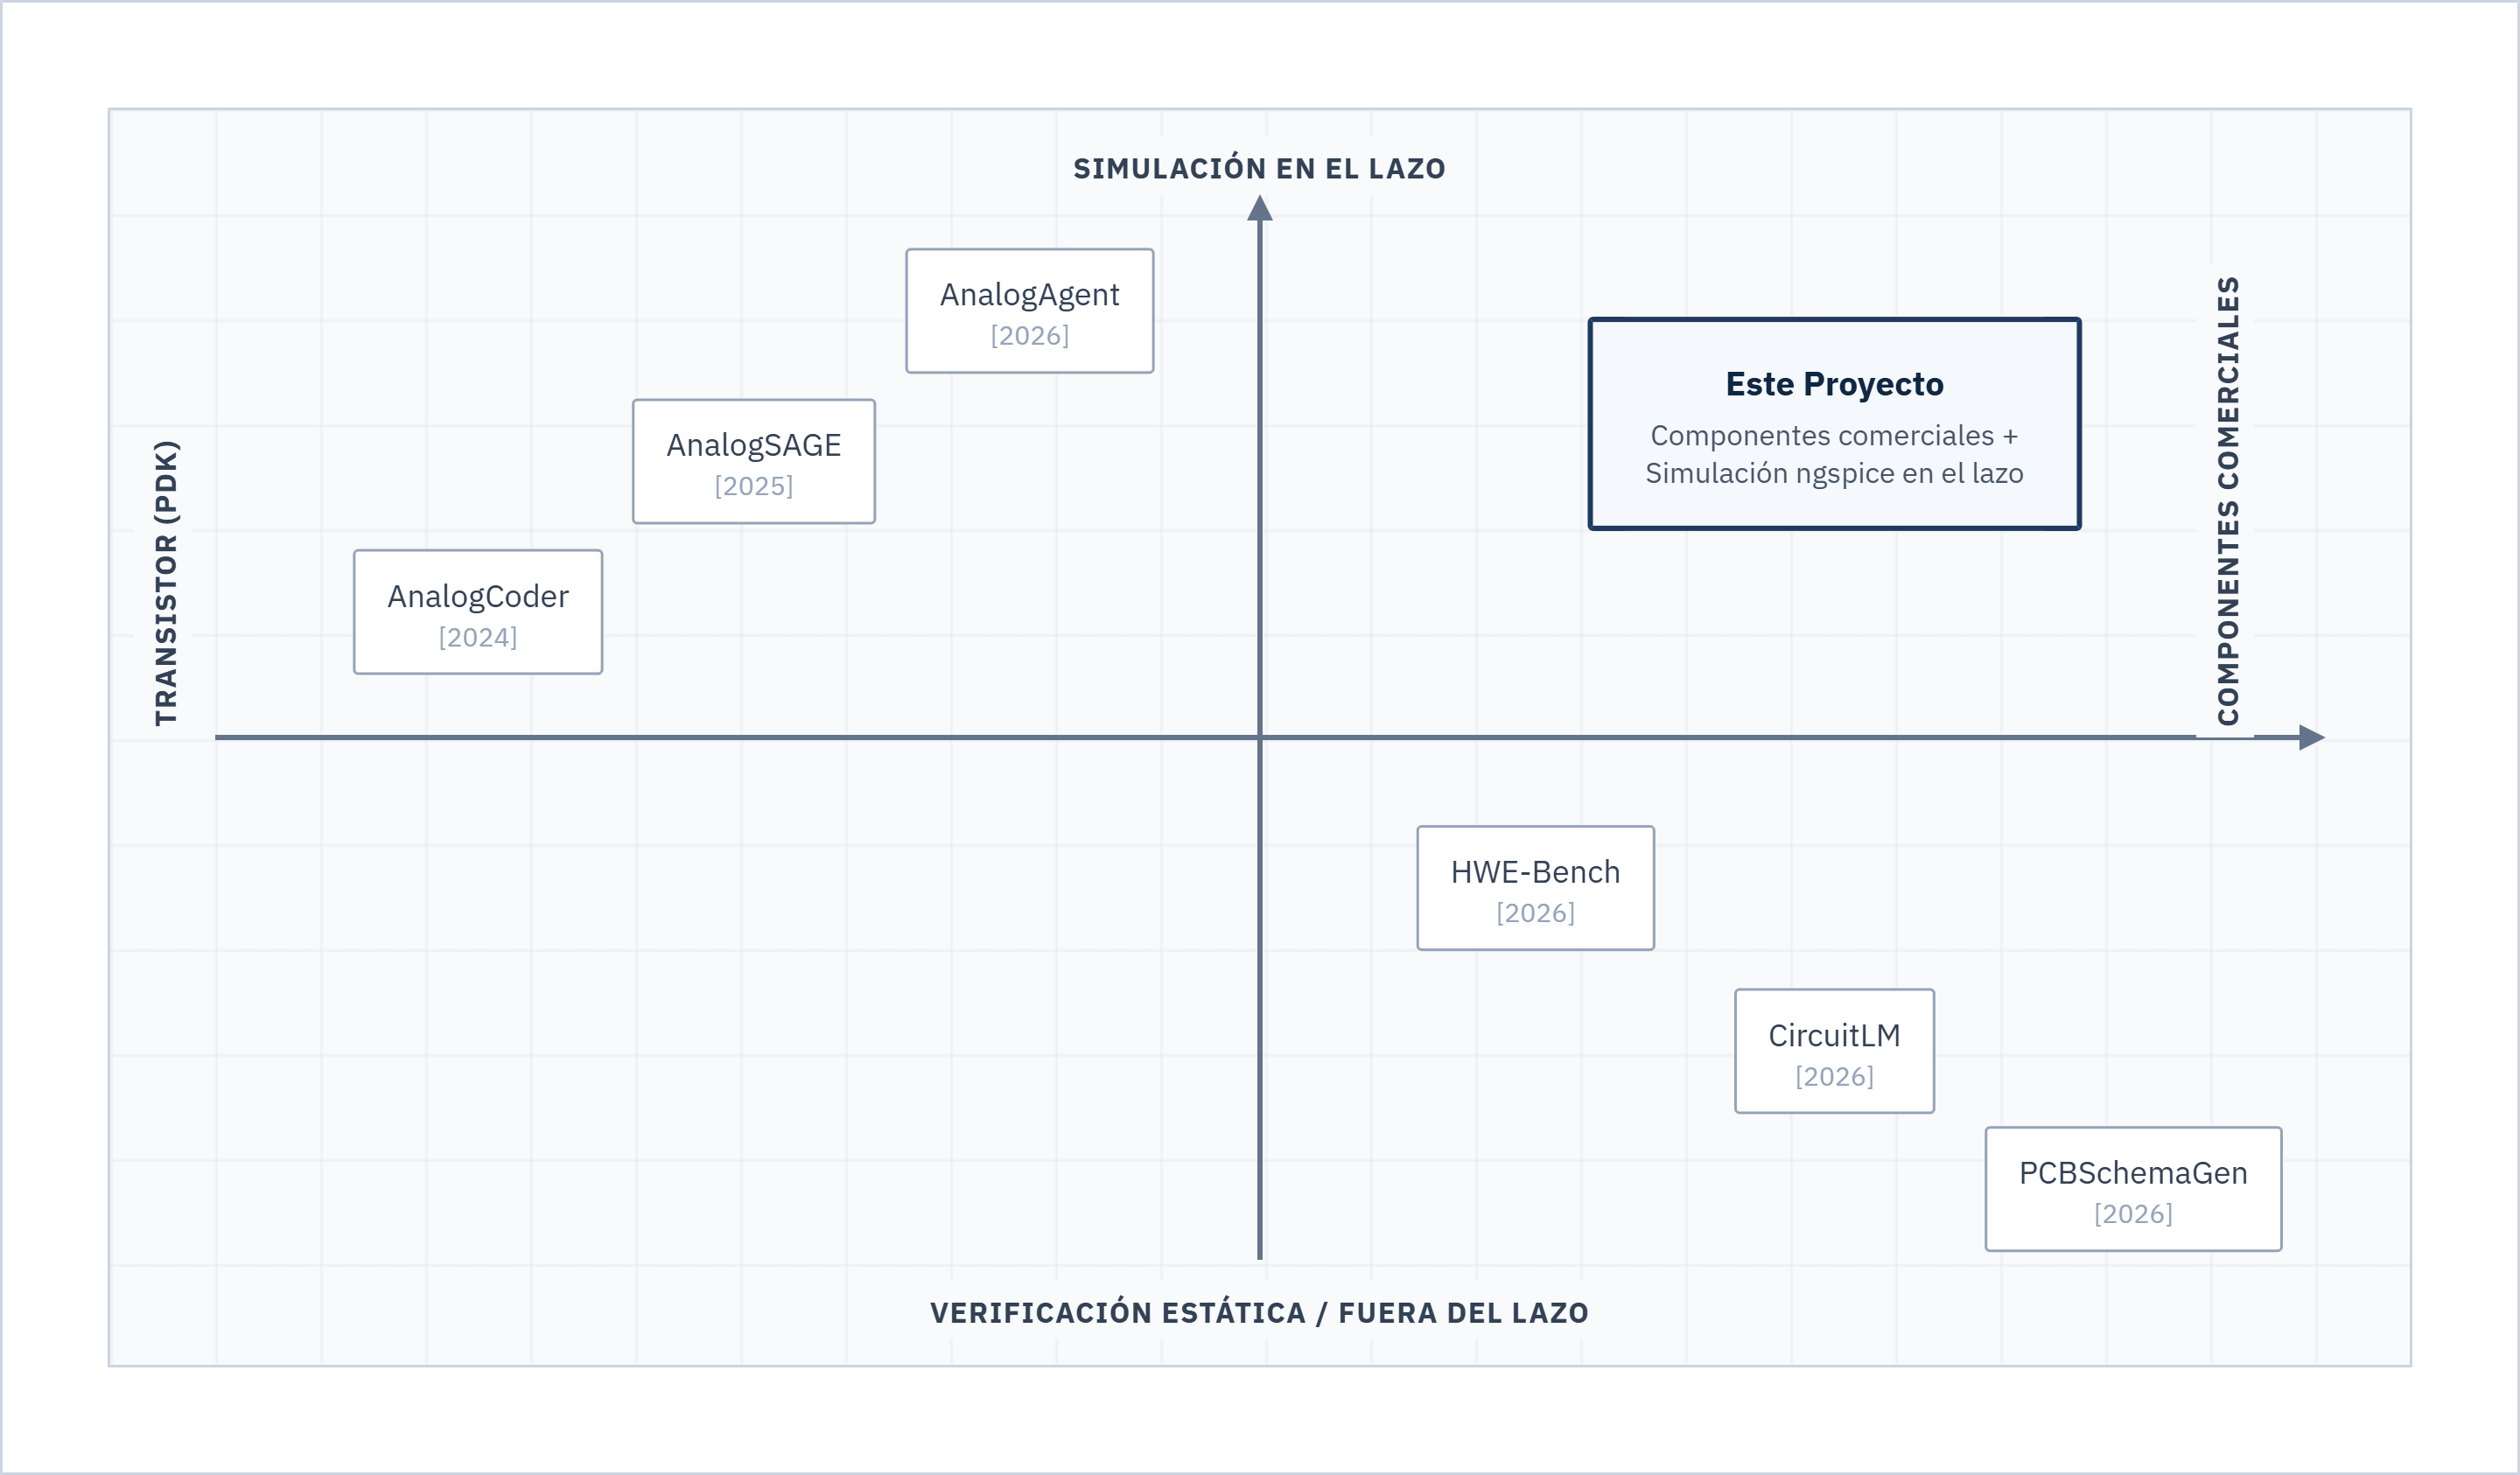
\includegraphics[width=1.2\textwidth, trim=0cm 0cm 0cm 0cm, clip]{../src/diagrams/edo_arte.png}%
    }
    \caption{Posición de los trabajos revisados según cuatro rasgos.}
    \label{fig:comparacion_estado_arte}
    \vspace{0.3cm}
\end{figure}

Junto a los desarrollos mencionados, otras propuestas complementan el panorama del área. \textbf{AnalogSAGE} \cite{analogsage} introduce memoria estratificada y mecanismos de autoevolución a la síntesis a nivel de transistor; \textbf{PCBSchemaGen} \cite{pcbschemagen} extiende la verificación estática de reglas al ámbito de tarjetas de circuito impreso reales; y \textbf{HWE-Bench} \cite{hwebench} provee un entorno de evaluación comparativa que mide el rendimiento de netlists generados contrastándolos con diseños de referencia de expertos a través de simulaciones SPICE. Adicionalmente, se registran contribuciones como \textbf{ADO-LLM} \cite{adollm} para la optimización bayesiana en el diseño físico y \textbf{SPICEPilot} \cite{spicepilot} para la generación asistida de scripts de control.

La Figura \ref{fig:comparacion_estado_arte} organiza los trabajos según los dos ejes que mejor los distinguen: el nivel de abstracción del diseño ---de transistor a componentes comerciales--- y la función de la simulación en el flujo ---de la verificación estática a la realimentación en el lazo---. El esquema de coordinación y el mecanismo de optimización paramétrica complementan el contraste y se desarrollan en el texto.

Al contrastar las soluciones se observa que ninguno de los antecedentes recopilados integra simultáneamente los cuatro rasgos propuestos en este ecosistema. Mientras que los sistemas orientados a transistores explotan la simulación en lazo cerrado y el ajuste paramétrico iterativo, no contemplan el uso de componentes comerciales. Por el contrario, los enfoques comerciales evitan la simulación dinámica en el lazo de optimización o la reducen a una métrica de prueba externa. Este proyecto une la retroalimentación física por simulación de los flujos a nivel de transistor con el diseño a nivel de placa mediante componentes comerciales, implementando una arquitectura multiagente coordinada por un curador entrenado por aprendizaje por refuerzo.


\begin{table}[h!]
\centering
\small
\label{tab:estado_del_arte}
\vspace{0.3cm}

\setlength{\aboverulesep}{0pt}
\setlength{\belowrulesep}{0pt}
\renewcommand{\arraystretch}{1.5}
\setlength{\extrarowheight}{5pt}
\arrayrulecolor{guinda}
\rowcolors{1}{white}{rowgray}

% Estructura rígida basada en tabularx con alineación vertical al centro
\begin{tabularx}{\textwidth}{
  >{\centering\arraybackslash}m{2.6cm} 
  >{\centering\arraybackslash}m{2.4cm} 
  >{\raggedright\arraybackslash}X 
  >{\centering\arraybackslash}m{1.5cm}
}
\toprule
\rowcolor{guinda}
\textcolor{white}{\textbf{Nombre del Paper}} & 
\textcolor{white}{\textbf{Origen}} & 
\textcolor{white}{\textbf{Descripción}} & 
\textcolor{white}{\textbf{Enlace}} \\ 
\midrule

AnalogCoder & 
\worldflag{HK} \worldflag{US} \newline \footnotesize HK / EE. UU. & 
Primer agente LLM sin entrenamiento para diseño de circuitos analógicos mediante generación de código Python y bibliotecas de subcircuitos. & 
\href{https://arxiv.org/abs/2405.14918}{\textbf{[Link]}} \\

AnalogAgent & 
\worldflag{SG} \newline \footnotesize Singapur & 
Arquitectura multi-agente con memoria auto-evolutiva que aprende de los fallos de simulación sin depender de bibliotecas externas. & 
\href{https://arxiv.org/abs/2603.23910}{\textbf{[Link]}} \\ 

CircuitLM & 
\worldflag{BD} \newline \footnotesize Bangladesh & 
Tubería multiagente que genera esquemas a nivel de placa con componentes comerciales, orientada a electrónica digital y embebida; valida con un motor de reglas eléctricas (ERC) y un modelo supervisor, sin simulación en el lazo. & 
\href{https://arxiv.org/abs/2601.04505}{\textbf{[Link]}} \\

\bottomrule
\end{tabularx}
\caption{Resumen - Estado del Arte}
\end{table}

  % CAPÍTULO 4: DISEÑO E IMPLEMENTACIÓN DE LA SOLUCIÓN
  \chapter{Diseño e Implementación de la Solución}
  % Capítulo 4: Propuesta de solución
\section{Introducción}
\label{sec:prop-intro}

En el capítulo anterior se revisó el estado del arte de los sistemas multiagente basados en LLM para el diseño de circuitos analógicos, y se identificó que los trabajos reportados operan a nivel de transistor sobre un nodo tecnológico (PDK), mientras que la generación y validación de circuitos a nivel de componentes comerciales (COTS) con simulación SPICE dentro del lazo de diseño permanece como una brecha abierta. Este capítulo presenta la propuesta de solución que atiende esa brecha.

El propósito del capítulo es exponer el diseño del sistema antes de su construcción: las premisas que lo fundamentan, su descomposición funcional, su arquitectura estructural y su comportamiento en ejecución. Las decisiones de diseño se justifican a partir de la naturaleza del problema, de los principios de la ingeniería de software y de los hallazgos del estado del arte; los artefactos de análisis y diseño elaborados a lo largo del proyecto —la Especificación de Requisitos de Software (SRS), el modelo de casos de uso, el diagrama funcional, el modelo arquitectónico C4 de tres niveles y el diagrama de secuencia— registran y representan esas decisiones, de modo que cada una quede expresada en un artefacto verificable.

La exposición sigue un orden de lo abstracto a lo concreto. Primero se establecen el problema que el diseño debe resolver, las premisas que lo orientan y el papel del SRS como registro de los requisitos (sección~\ref{sec:prop-premisas}). A continuación se describe \textit{qué} hace el sistema mediante su descomposición funcional y sus casos de uso (sección~\ref{sec:prop-funcional}). Después se describe \textit{cómo} se estructura, mediante el modelo C4 en sus tres niveles (sección~\ref{sec:prop-c4}). Enseguida se describe \textit{cómo se comporta} en ejecución, mediante el diagrama de secuencia del flujo principal de generación (sección~\ref{sec:prop-dinamico}). Finalmente se explican los atributos de calidad y seguridad que se desprenden del diseño (secciones~\ref{sec:prop-calidad} y~\ref{sec:prop-seguridad}), se enuncian los criterios de aceptación que la propuesta deberá satisfacer (sección~\ref{sec:prop-criterios}) y se cierra con una síntesis del diseño y su conexión con la evaluación del sistema (sección~\ref{sec:prop-sintesis}).

\section{Premisas y fundamento de diseño}
\label{sec:prop-premisas}

\subsection{El problema de diseño y el papel del SRS}
\label{subsec:prop-problema}

El diseño responde a un problema concreto: transformar la descripción de un circuito analógico CA/CD, expresada en lenguaje natural, en un netlist que haya sido simulado y validado, empleando componentes comerciales en lugar de dispositivos a nivel de transistor. Este problema impone por sí mismo varias exigencias al diseño —la interpretación de lenguaje natural, el cálculo de valores de componentes, la simulación física y el ajuste del circuito hasta cumplir una meta— que son las que, en última instancia, justifican la forma del sistema. Las decisiones de diseño de este capítulo se fundamentan en esas exigencias del problema, en los principios de la ingeniería de software y en los hallazgos del estado del arte, y no en la conformidad con un documento interno.

La Especificación de Requisitos de Software (SRS) en su versión 1.0 cumple un papel distinto al de fuente de justificación: es el artefacto que registra de forma ordenada y verificable los requisitos que el sistema debe satisfacer, los traduce a criterios de verificación y delimita el alcance. El SRS fija qué se construye —el alcance, los requisitos funcionales por subsistema, los requisitos no funcionales y los criterios de aceptación—; las razones por las que el diseño adopta una u otra forma se exponen en este capítulo a partir del problema y de la disciplina, y los identificadores de requisito (RF, RNF) se citan únicamente para señalar qué requisito queda cubierto por cada decisión, no para sustentarla.

El alcance del sistema comprende recibir la descripción de un circuito analógico en lenguaje natural, dividir circuitos de varias etapas en sub-bloques, calcular los valores de los componentes, generar el código PySpice y el netlist, simular en ngspice, ajustar iterativamente los valores mediante un agente curador, y entregar al usuario el netlist final junto con las métricas y el historial de iteraciones. Quedan fuera del alcance el diseño de \textit{layout} físico (PCB), la síntesis a nivel de transistor para un nodo tecnológico y la generación de esquemáticos gráficos.

\subsection{Premisas de diseño}
\label{subsec:prop-premisas-disenio}

A partir del problema descrito, y guiado por principios reconocidos de la ingeniería de software, el diseño adopta un conjunto de premisas que orientan las decisiones arquitectónicas de las secciones siguientes. Para cada una se expone primero su fundamento y, después, el requisito del SRS que queda cubierto.

La primera premisa es la separación del sistema en dos subsistemas que se despliegan por separado. Esta decisión aplica el principio de separación de intereses: las responsabilidades de acceso —autenticación, sesiones, espacios de trabajo y emisión de API keys— pertenecen a un dominio distinto del de la generación de circuitos, y mantenerlas en subsistemas separados reduce el acoplamiento entre ambos y permite desplegarlos, escalarlos y razonar sobre ellos de forma independiente. De ahí que el subsistema cliente actúe como puerta de entrada de los usuarios y no ejecute lógica de diseño de circuitos, que reside íntegramente en el subsistema servidor.

Dentro del servidor, el diseño se rige por la modularidad de los agentes, que materializa los principios de alta cohesión y bajo acoplamiento: cada agente concentra una responsabilidad única y se comunica con los demás solo a través de un estado compartido, sin conocer su implementación interna. Esta organización permite reemplazar o modificar un agente sin alterar los restantes, propiedad que la literatura sobre sistemas multiagente para diseño de circuitos asocia con la capacidad de evolucionar y depurar cada agente por separado, y que en el SRS queda recogida como requisito de mantenibilidad (RNF-04.1).

A esta modularidad se suma la concurrencia en el cálculo, que no es una decisión arbitraria sino una consecuencia de la estructura del problema: un circuito de varias etapas se descompone en sub-bloques, y aquellos que no dependen entre sí pueden calcularse de forma simultánea sin afectar el resultado. El diseño aprovecha esta independencia mediante un patrón Master-Worker con \textit{Map-Reduce}, en el que un nodo Master reparte cada sub-bloque independiente como tarea a un worker y luego recombina los resultados. Esta correspondencia entre la naturaleza paralelizable del problema y la estructura concurrente del sistema queda cubierta por los requisitos de reparto y desempeño del SRS (RF-01.3, RNF-01.2).

El rasgo que distingue la propuesta frente a los enfoques revisados en el estado del arte es la validación dentro del lazo de diseño. Los sistemas multiagente reportados para diseño analógico tienden a emplear la simulación como comprobación posterior a la generación; la propuesta, en cambio, la incorpora como parte del proceso de ajuste: el agente curador compara las métricas obtenidas de ngspice con las metas y decide si el circuito se acepta o se vuelve a ajustar, hasta cumplir la meta o alcanzar un número máximo de iteraciones. Esta integración de la simulación en el lazo es la traducción, al nivel de componentes comerciales, del cierre de realimentación que la literatura sobre diseño asistido por LLM ha mostrado eficaz al nivel de transistor, y constituye la aportación central de la propuesta; en el SRS se recoge como el control del ciclo de ajuste (RF-01.4).

Sostener ese lazo exige conservar el estado entre iteraciones, por lo que el diseño conserva de forma explícita el estado de la generación mediante un mecanismo de \textit{checkpointer} sobre una base de datos, de modo que una solicitud en proceso mantenga su estado disponible para todos los agentes a lo largo de las iteraciones. Esta persistencia se modela de manera explícita en el comportamiento dinámico del sistema (sección~\ref{sec:prop-dinamico}) por ser una propiedad esencial del lazo, y no una nota accesoria. Finalmente, y en línea con el principio de configurabilidad sin recompilación, los parámetros del agente curador —los pesos, factores y umbrales del cálculo de recompensa, junto con el número máximo de iteraciones— se mantienen en un archivo de configuración externo, de modo que puedan ajustarse durante la experimentación sin modificar el código (RNF-04.2).

% FIGURA 4.1 — Mapa de cobertura: decisiones de diseño ↔ requisitos.
% (referencia pendiente: añadir `mapa_cobertura.png` en src/diagrams si procede)

\section{Descomposición funcional y casos de uso}
\label{sec:prop-funcional}

\subsection{Vista funcional}
\label{subsec:prop-vista-funcional}

El sistema ofrece un conjunto acotado de funciones que se desprenden directamente del problema y quedan registradas en el SRS: dar acceso a los usuarios y gestionar sus sesiones, espacios de trabajo y API keys (cliente); leer una descripción de circuito en lenguaje natural y extraer de ella los parámetros eléctricos; dividir un circuito de varias etapas en sub-bloques; calcular los valores de los componentes de cada sub-bloque; generar el código PySpice y el netlist; simular el netlist en ngspice y leer las métricas; comparar las métricas con las metas y decidir si el circuito se acepta o se ajusta; y entregar al usuario el netlist final junto con las métricas y el historial de iteraciones.

El diagrama funcional organiza estas funciones según el subsistema responsable y el flujo de datos que las relaciona, lo que permite ver la propuesta como un encadenamiento de transformaciones sobre la descripción del circuito, desde el lenguaje natural hasta el netlist validado.

\begin{figure}[H]
    \centering
    \makebox[\textwidth][c]{%
        \hspace*{-0.5cm}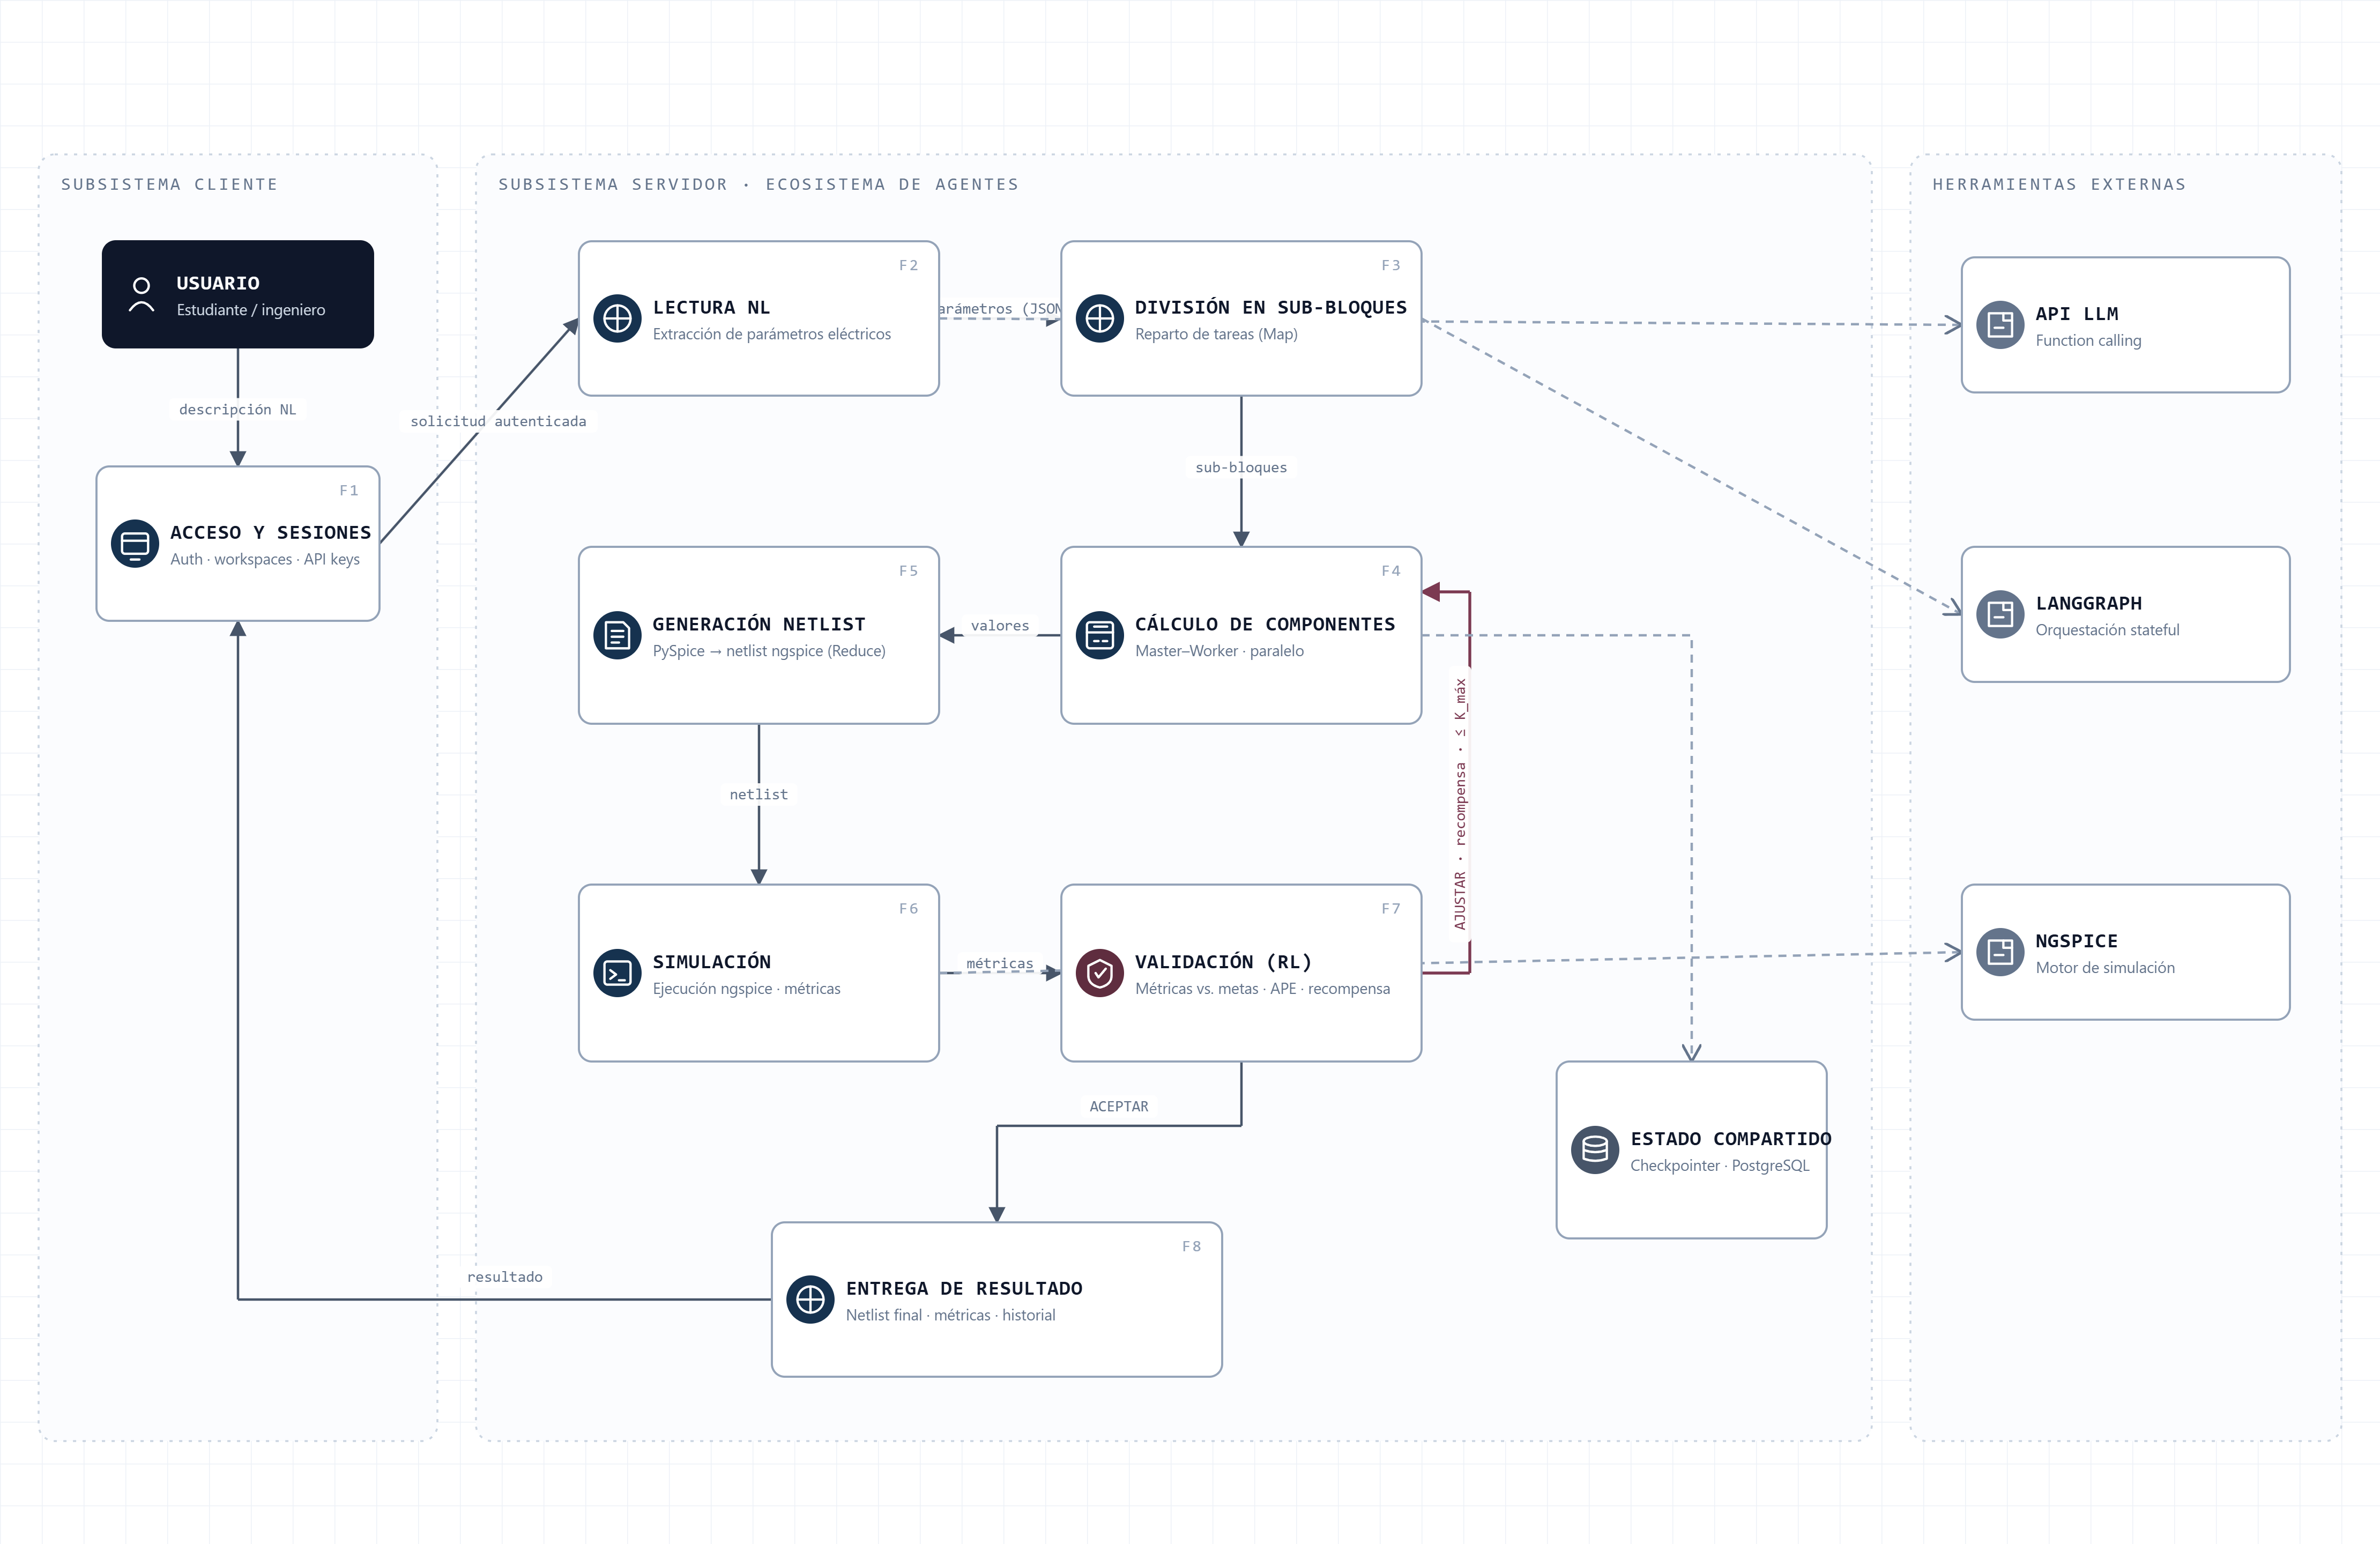
\includegraphics[width=1.3\textwidth, keepaspectratio]{../src/diagrams/diagrama_funcional.png}%
    }
    \caption{Diagrama funcional del sistema.}
    \label{fig:diagrama-funcional}
\end{figure}

\subsection{Modelo de casos de uso}
\label{subsec:prop-casos-uso}

Los casos de uso describen las interacciones que los actores ejecutan sobre el sistema. Se identifican dos clases de actor: el \textbf{usuario}, que interactúa con el subsistema cliente, y los \textbf{servicios externos} (la API del LLM y el motor ngspice), que el subsistema servidor consume durante la generación.

Los casos de uso principales del usuario incluyen: registrarse e iniciar sesión, gestionar espacios de trabajo, emitir y revocar API keys, y enviar una solicitud de generación de circuito junto con su descripción en lenguaje natural. El caso de uso central —\textit{generar circuito}— desencadena el flujo del subsistema servidor, que se detalla en su comportamiento dinámico en (sección~\ref{sec:prop-dinamico}). Los diagramas de casos de uso restantes (acceso, generación y decisión) se incluyen en el apéndice~\ref{apend:casos-uso}.

\begin{figure}[H]
    \centering
    \makebox[\textwidth][c]{%
        \hspace*{-0.5cm}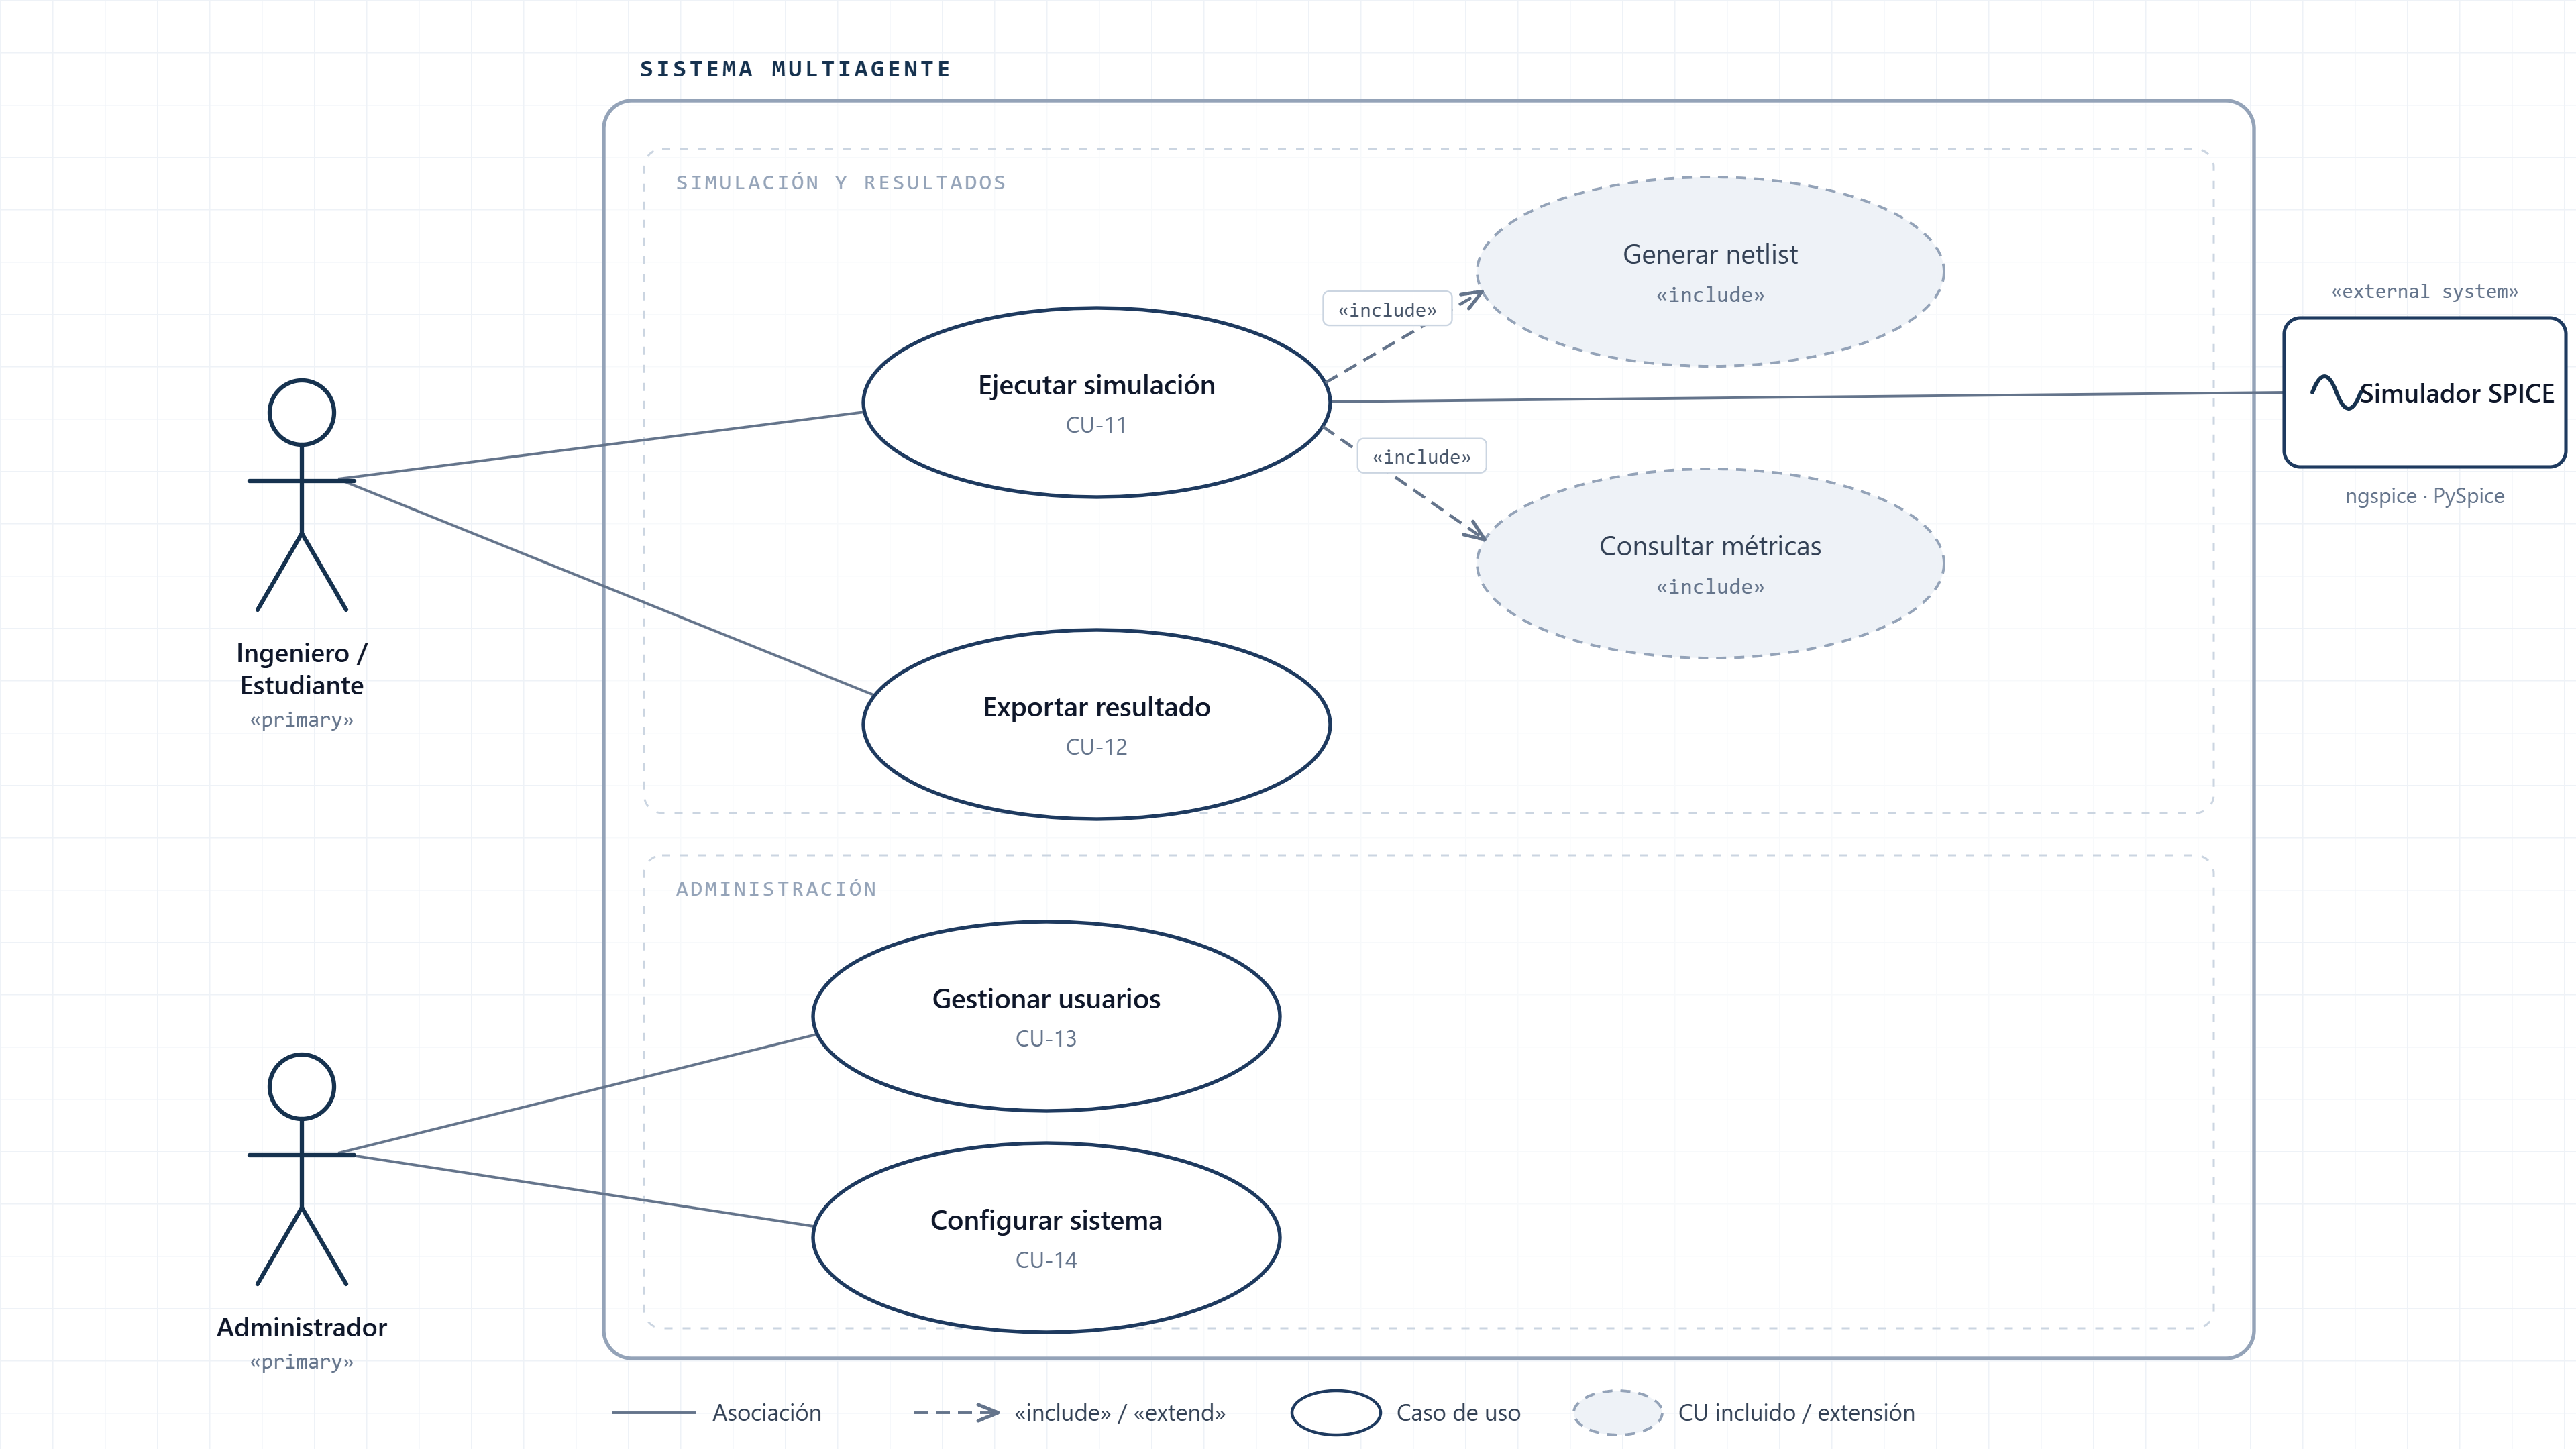
\includegraphics[width=1.3\textwidth, keepaspectratio]{../src/diagrams/casos_uso_simulacion.png}%
    }
    \caption{Diagrama de casos de uso: flujo de simulación y validación.}
    \label{fig:casos-uso-simulacion}
\end{figure}

\section{Arquitectura del sistema (modelo C4)}
\label{sec:prop-c4}

\subsection{Nivel 1 — Contexto}
\label{subsec:prop-c4-nivel1}

El nivel de contexto sitúa el sistema frente a sus actores y sistemas externos. Muestra al usuario interactuando con el sistema, y al sistema consumiendo dos servicios externos: la API del LLM y el motor de simulación ngspice. Este nivel deja claro que el sistema es una unidad que media entre la intención del usuario, expresada en lenguaje natural, y dos capacidades externas: el razonamiento del LLM y la simulación física del circuito.

\begin{figure}[H]
    \centering
    \makebox[\textwidth][c]{%
        \hspace*{-0.5cm}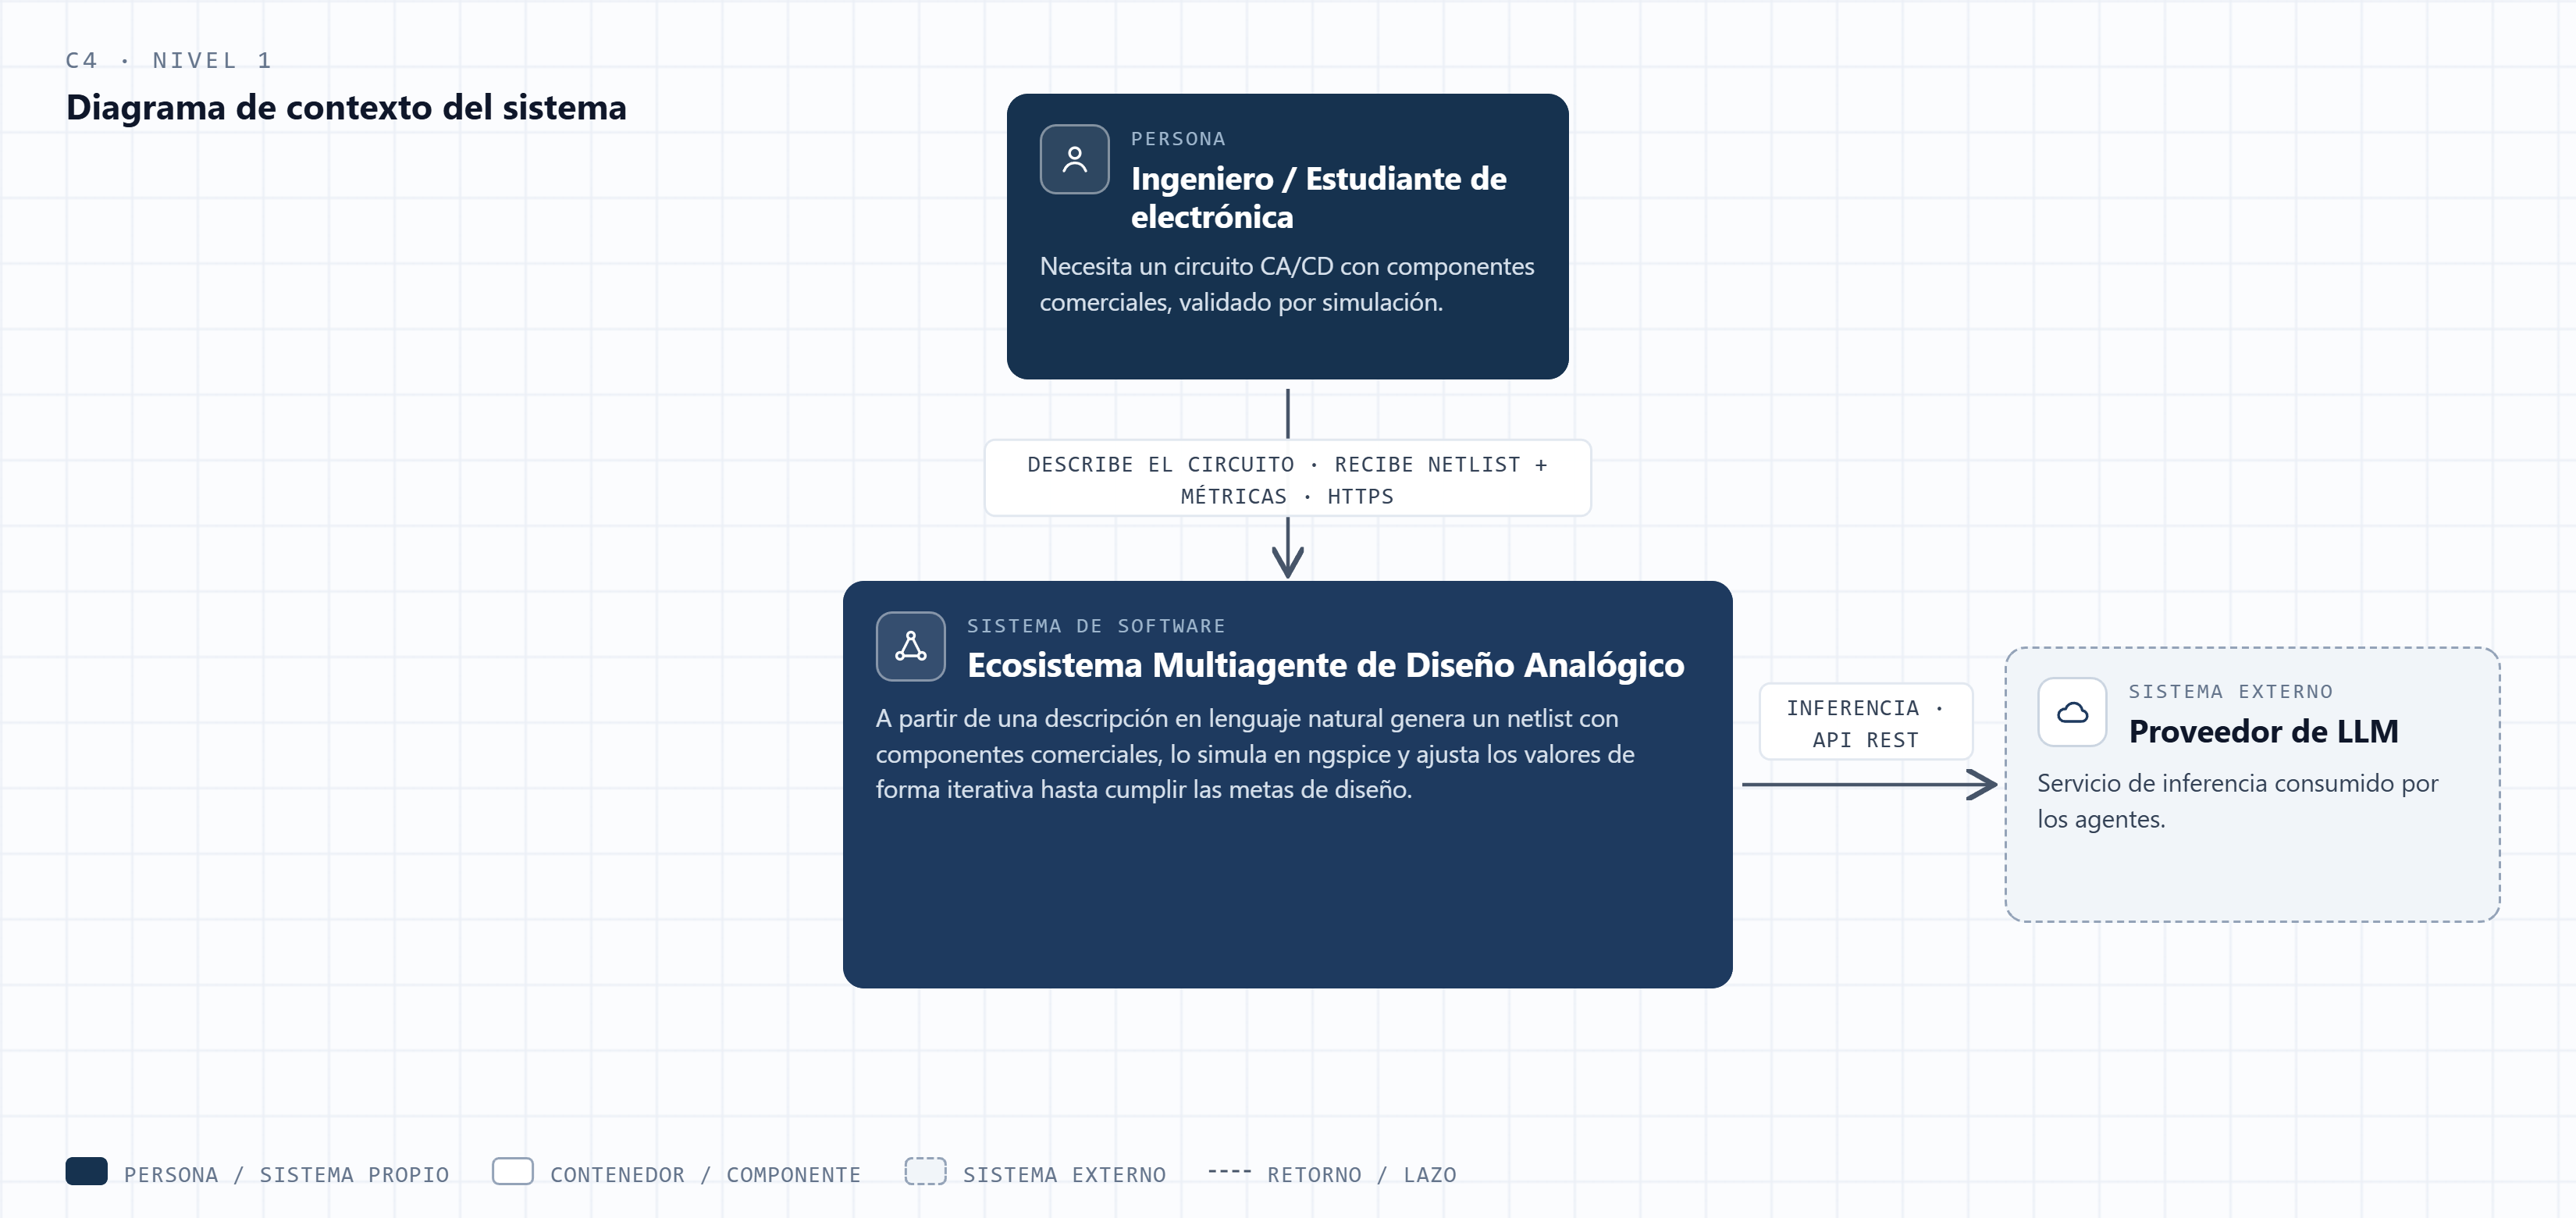
\includegraphics[width=1.3\textwidth, keepaspectratio]{../src/diagrams/c4_l1_v4.png}%
    }
    \caption{C4 Nivel 1: Diagrama de contexto.}
    \label{fig:c4-nivel1}
\end{figure}

\subsection{Nivel 2 — Contenedores}
\label{subsec:prop-c4-nivel2}

El nivel de contenedores descompone el sistema en sus unidades desplegables. Hace explícita la separación cliente/servidor: el subsistema cliente (autenticación, sesiones, espacios de trabajo, API keys) y el subsistema servidor (el ecosistema de agentes), junto con la base de datos de persistencia y la frontera con los servicios externos. Este nivel justifica la premisa de despliegue independiente (sección~\ref{subsec:prop-premisas-disenio}) y muestra el camino de una solicitud autenticada desde el cliente hacia el servidor.

\begin{figure}[H]
    \centering
    \makebox[\textwidth][c]{%
        \hspace*{-0.5cm}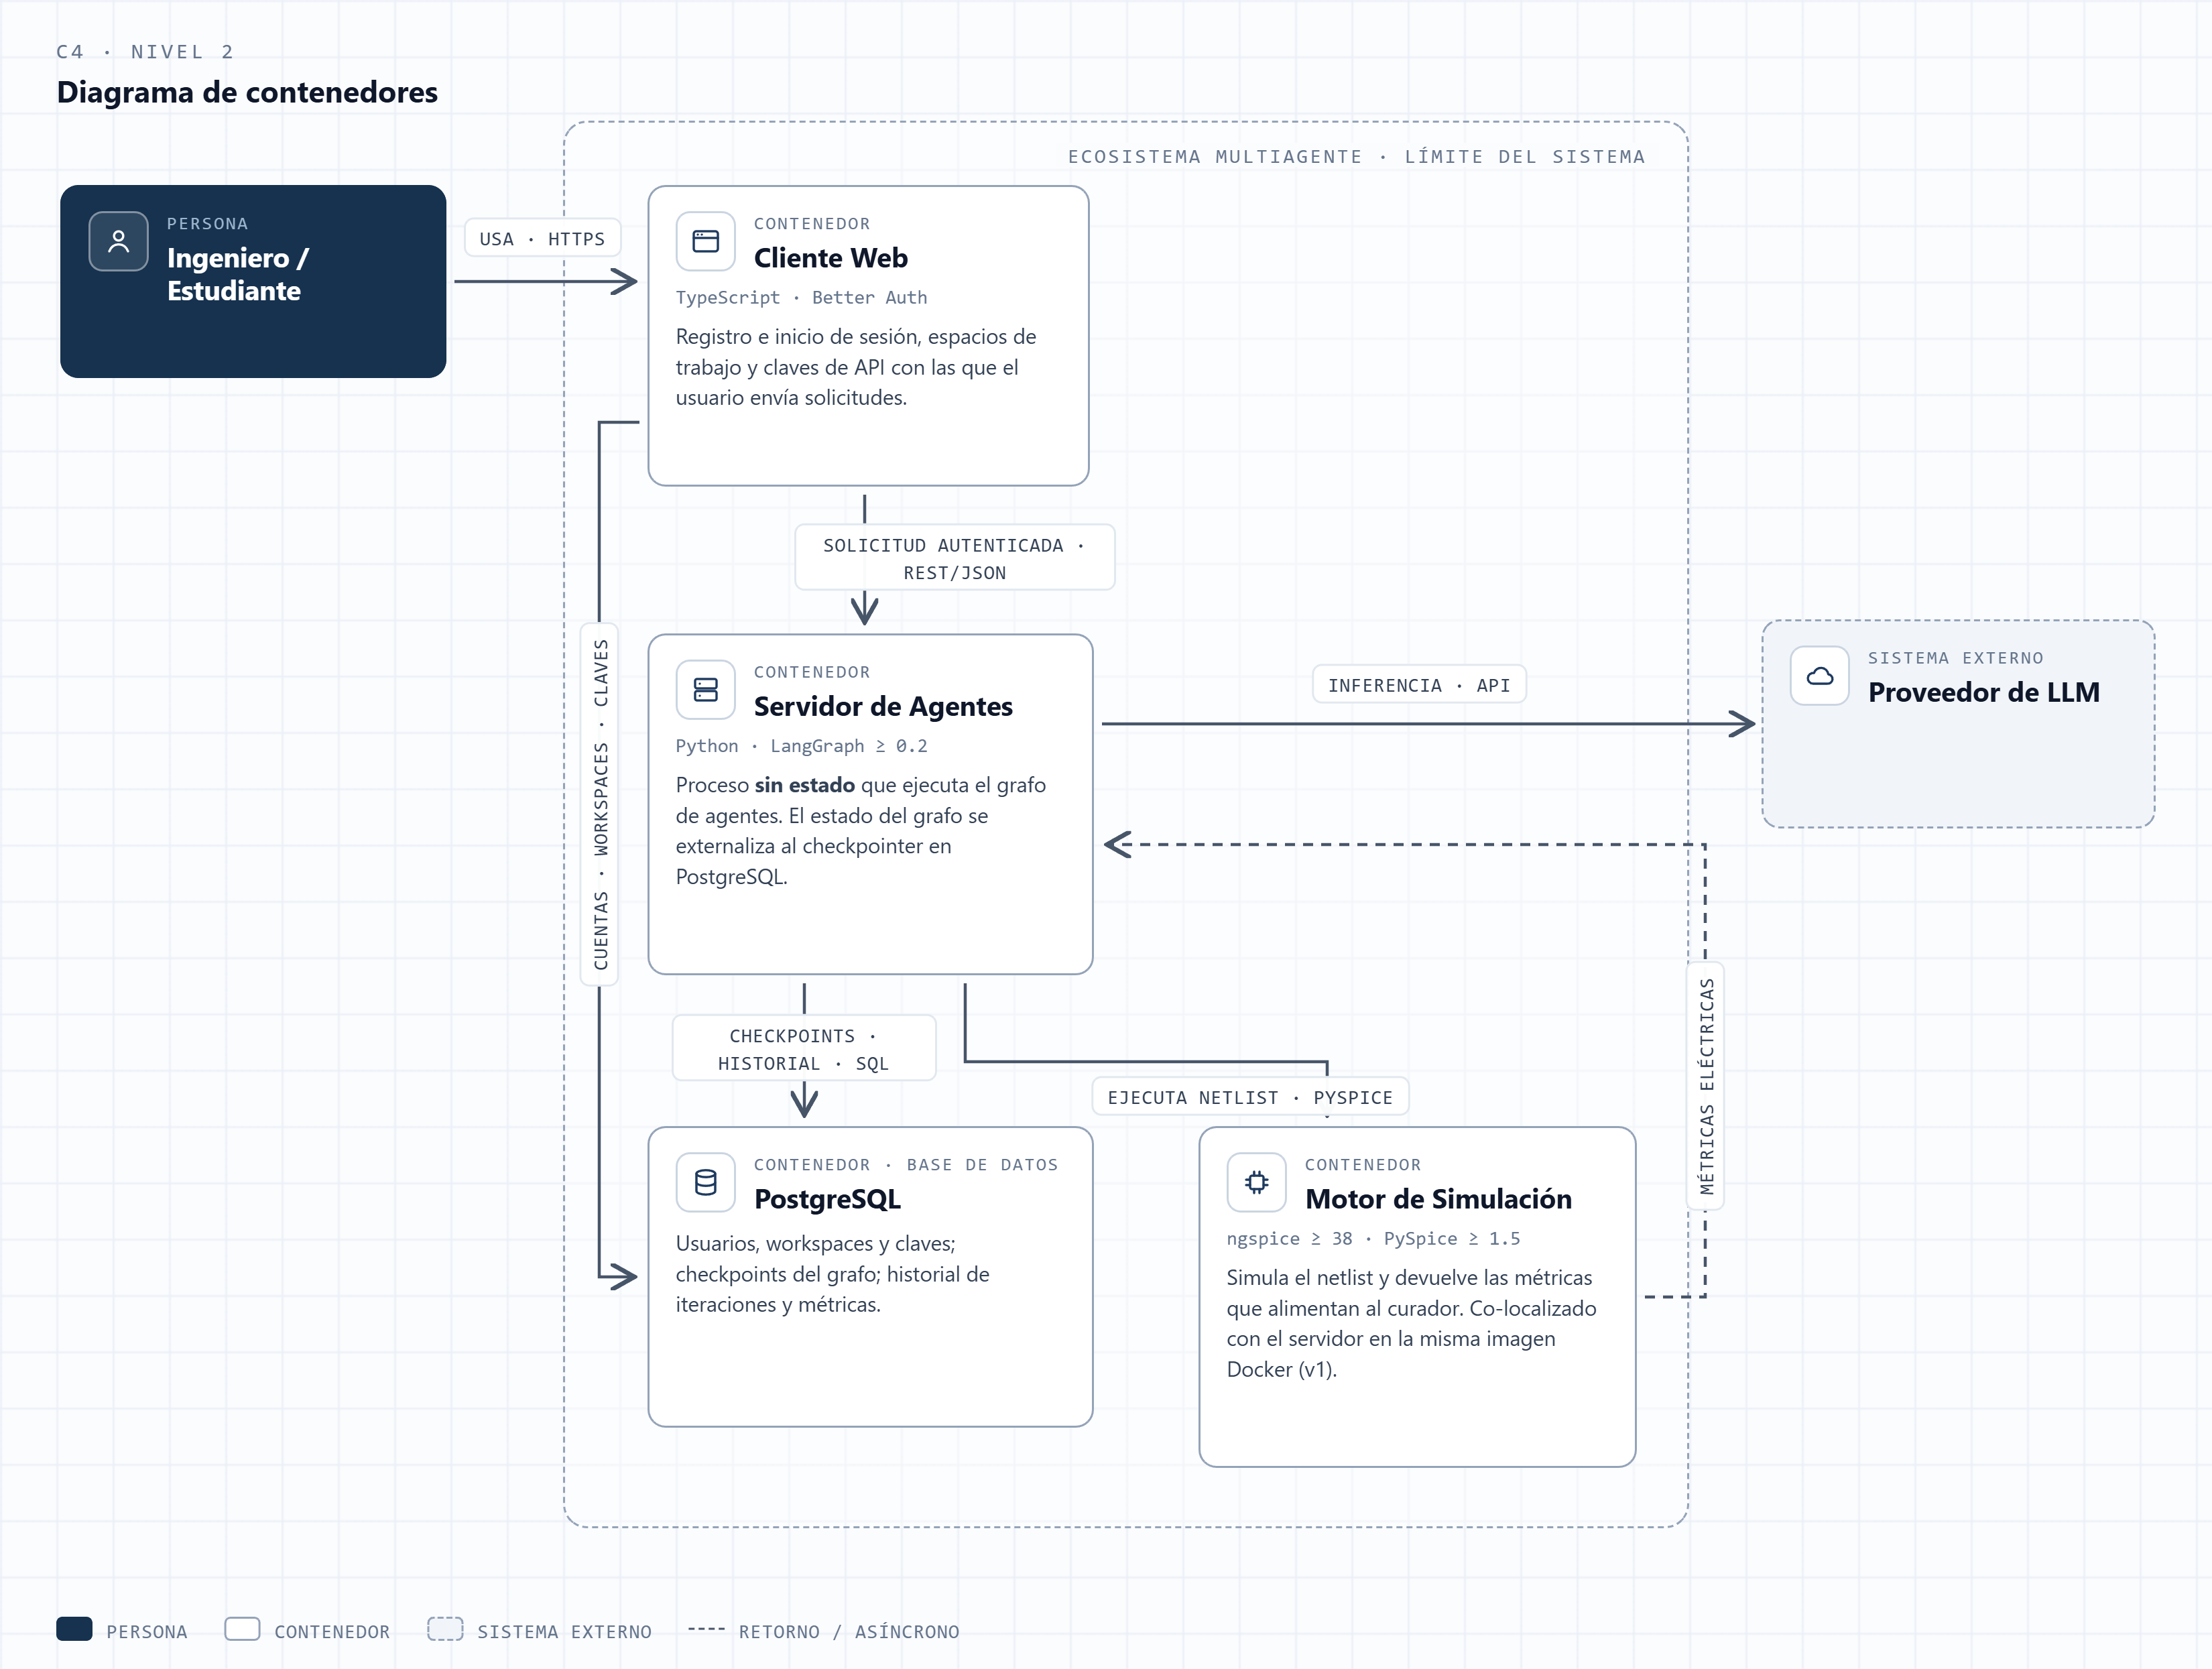
\includegraphics[width=1.3\textwidth, keepaspectratio]{../src/diagrams/c4_l2_v4.png}%
    }
    \caption{C4 Nivel 2: Diagrama de contenedores.}
    \label{fig:c4-nivel2}
\end{figure}

\subsection{Nivel 3 — Componentes}
\label{subsec:prop-c4-nivel3}

El nivel de componentes abre el subsistema servidor y muestra el ecosistema de agentes: el agente Orquestador (entrada del servidor y coordinador del estado compartido), el agente de Cálculo (Master-Worker), el agente Curador (RL, lazo de validación iterativa), el agente de Shell (ejecución de ngspice) y el agente de Escritura (generación del netlist con PySpice), todos coordinados sobre el grafo de orquestación con persistencia en base de datos. Este nivel materializa la premisa de modularidad de agentes (sección~\ref{subsec:prop-premisas-disenio}) y prepara el terreno para la descripción del comportamiento dinámico.

\begin{figure}[H]
    \centering
    \makebox[\textwidth][c]{%
        \hspace*{-0.5cm}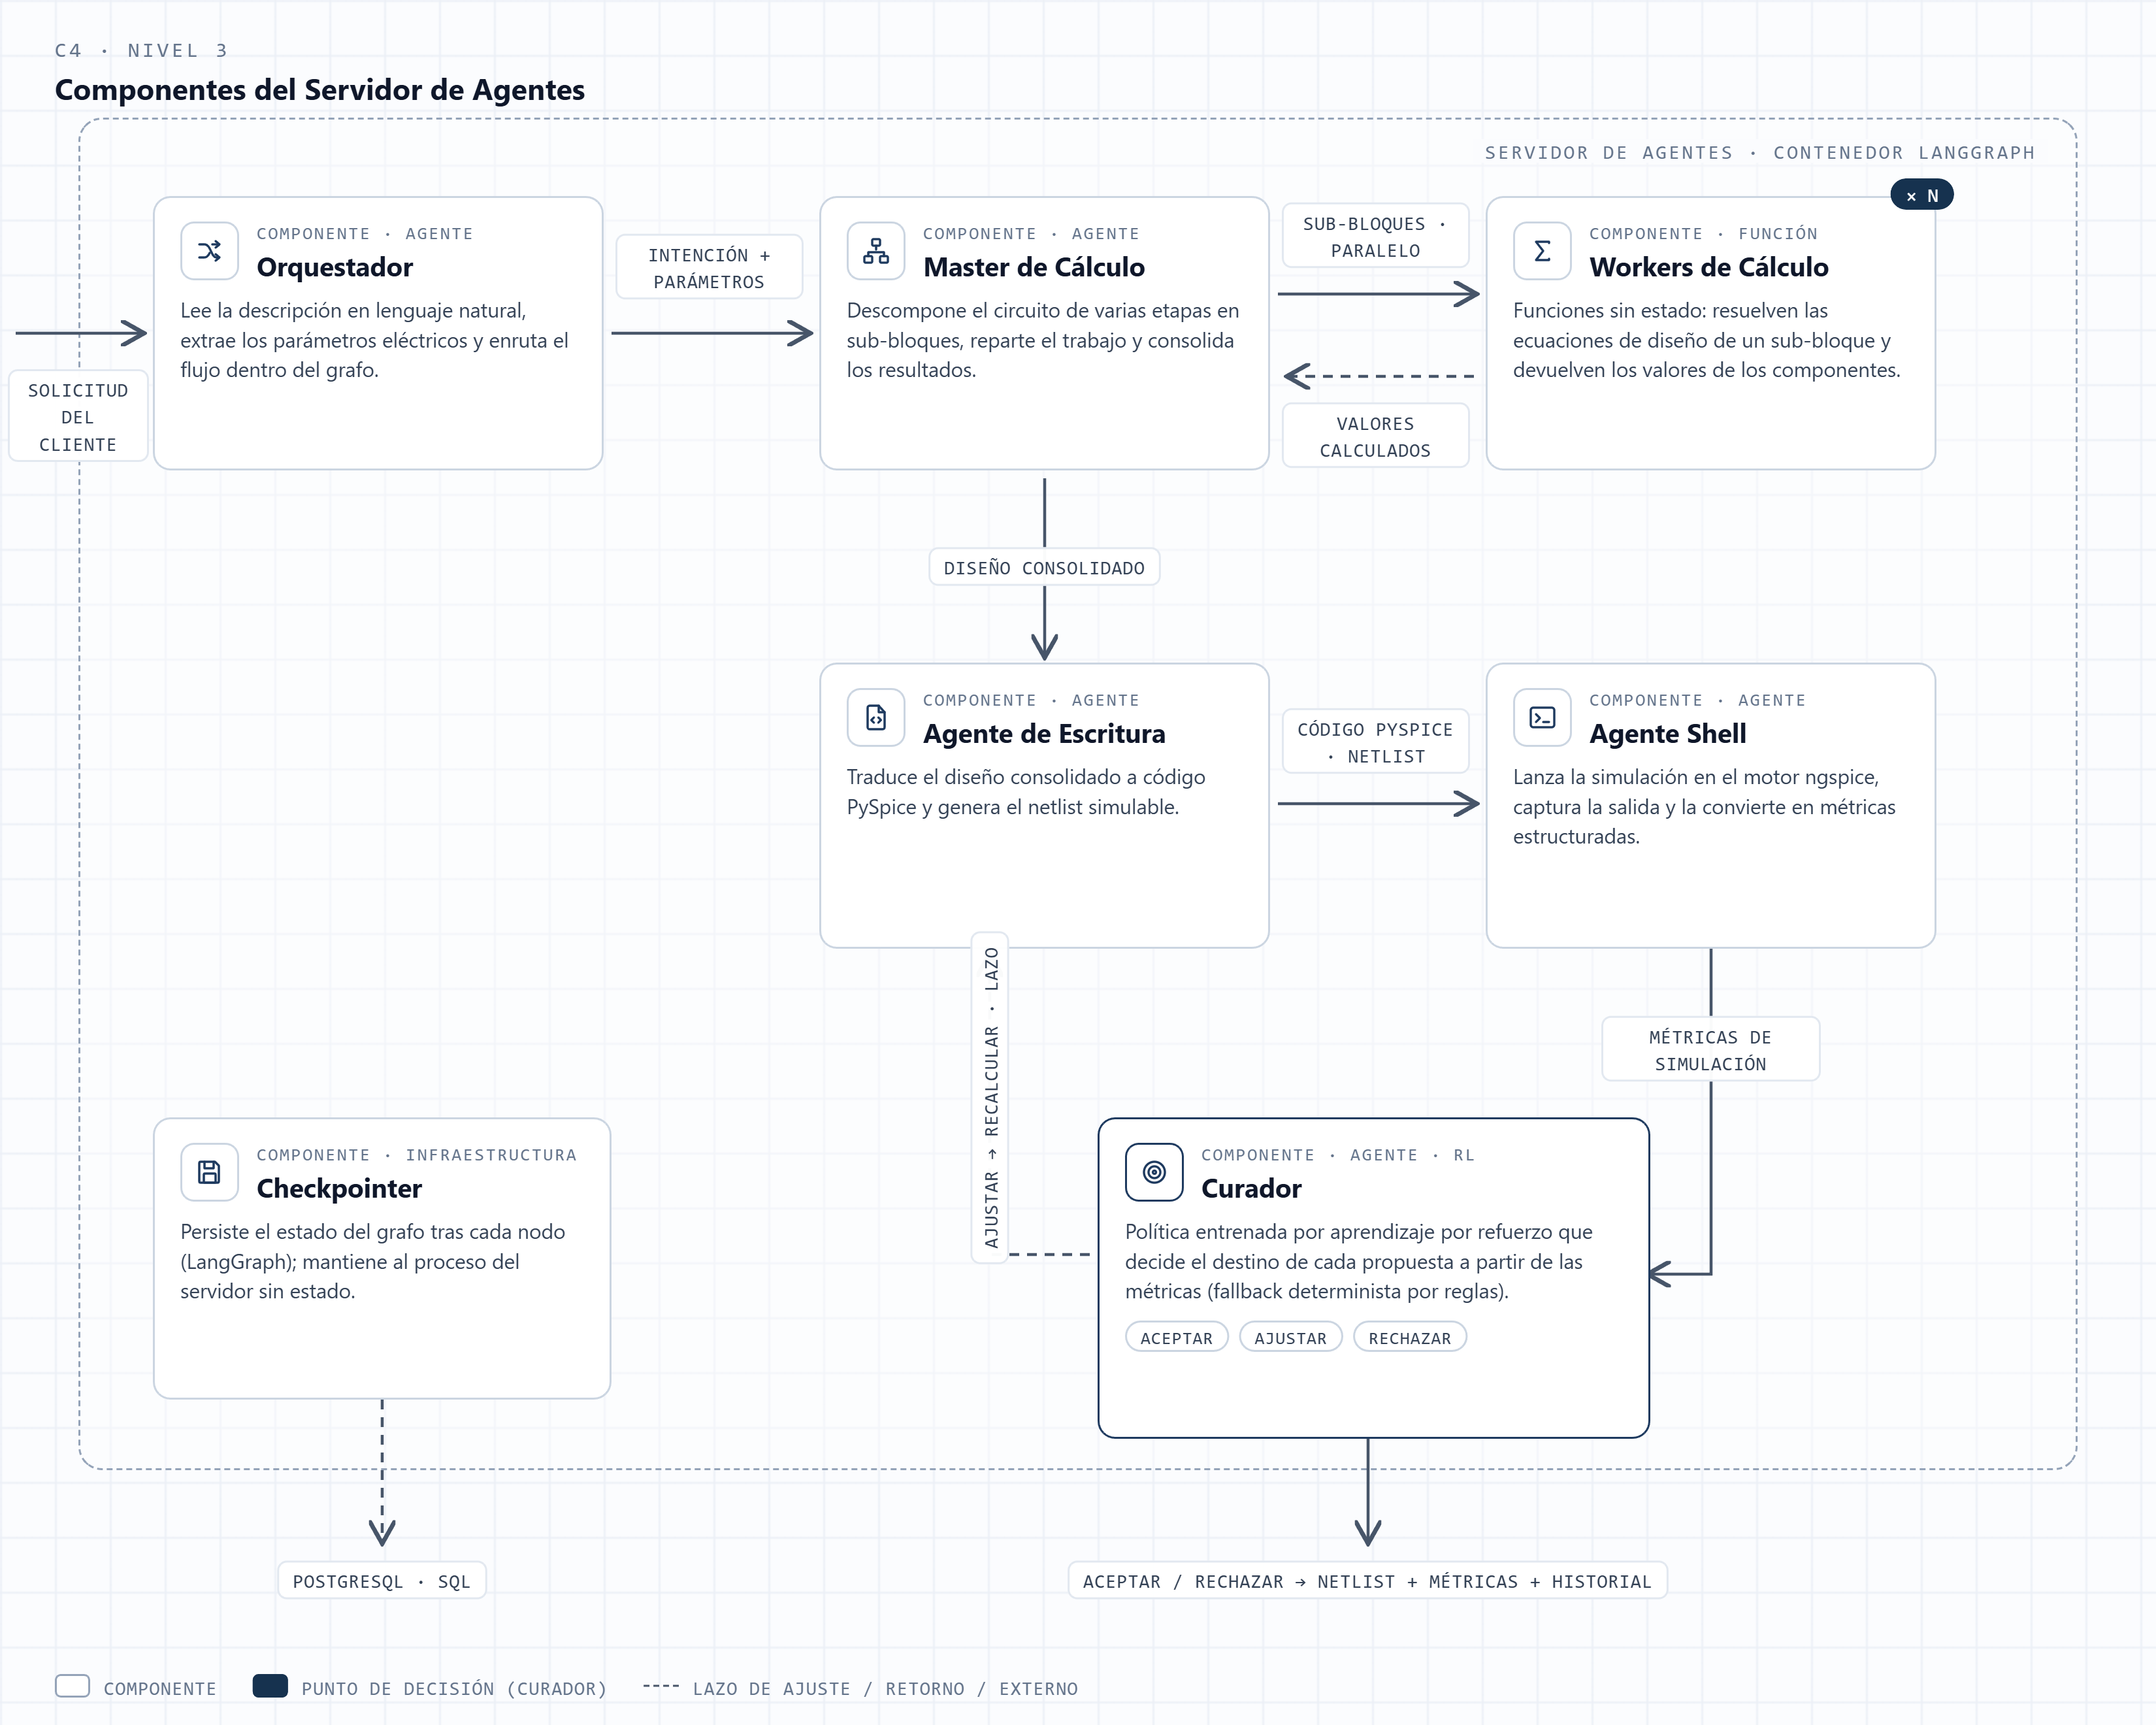
\includegraphics[width=1.3\textwidth, keepaspectratio]{../src/diagrams/c4_l3_v4.png}%
    }
    \caption{C4 Nivel 3: Diagrama de componentes.}
    \label{fig:c4-nivel3}
\end{figure}

\section{Comportamiento dinámico: flujo de generación}
\label{sec:prop-dinamico}

Las secciones anteriores describen la estructura estática del sistema. Esta sección describe su comportamiento en ejecución: cómo colaboran los agentes en el tiempo para transformar una descripción en lenguaje natural en un netlist validado. El diagrama de secuencia integra las vistas anteriores en una línea temporal.

El flujo principal procede así: el orquestador recibe la solicitud autenticada y la descripción del circuito, usa el LLM para extraer los parámetros y la lista de sub-bloques, y reparte los sub-bloques independientes en paralelo al agente de cálculo (Master-Worker). El agente de escritura genera el código PySpice y el netlist; el agente de shell lo simula en ngspice y lee las métricas; el agente curador compara las métricas con las metas y decide. Según su decisión, el ciclo se repite —ajustando los valores— o termina. El ciclo está acotado por un número máximo de iteraciones configurable (parámetro de guarda del lazo).

El comportamiento de persistencia se modela de forma explícita: el estado de cada iteración se conserva mediante el \textit{checkpointer}, lo que se representa como un fragmento de referencia en el diagrama, de modo que la naturaleza con estado del sistema quede formalmente reflejada y no como una observación accesoria.

\begin{figure}[H]
    \centering
    \makebox[\textwidth][c]{%
        \hspace*{-0.5cm}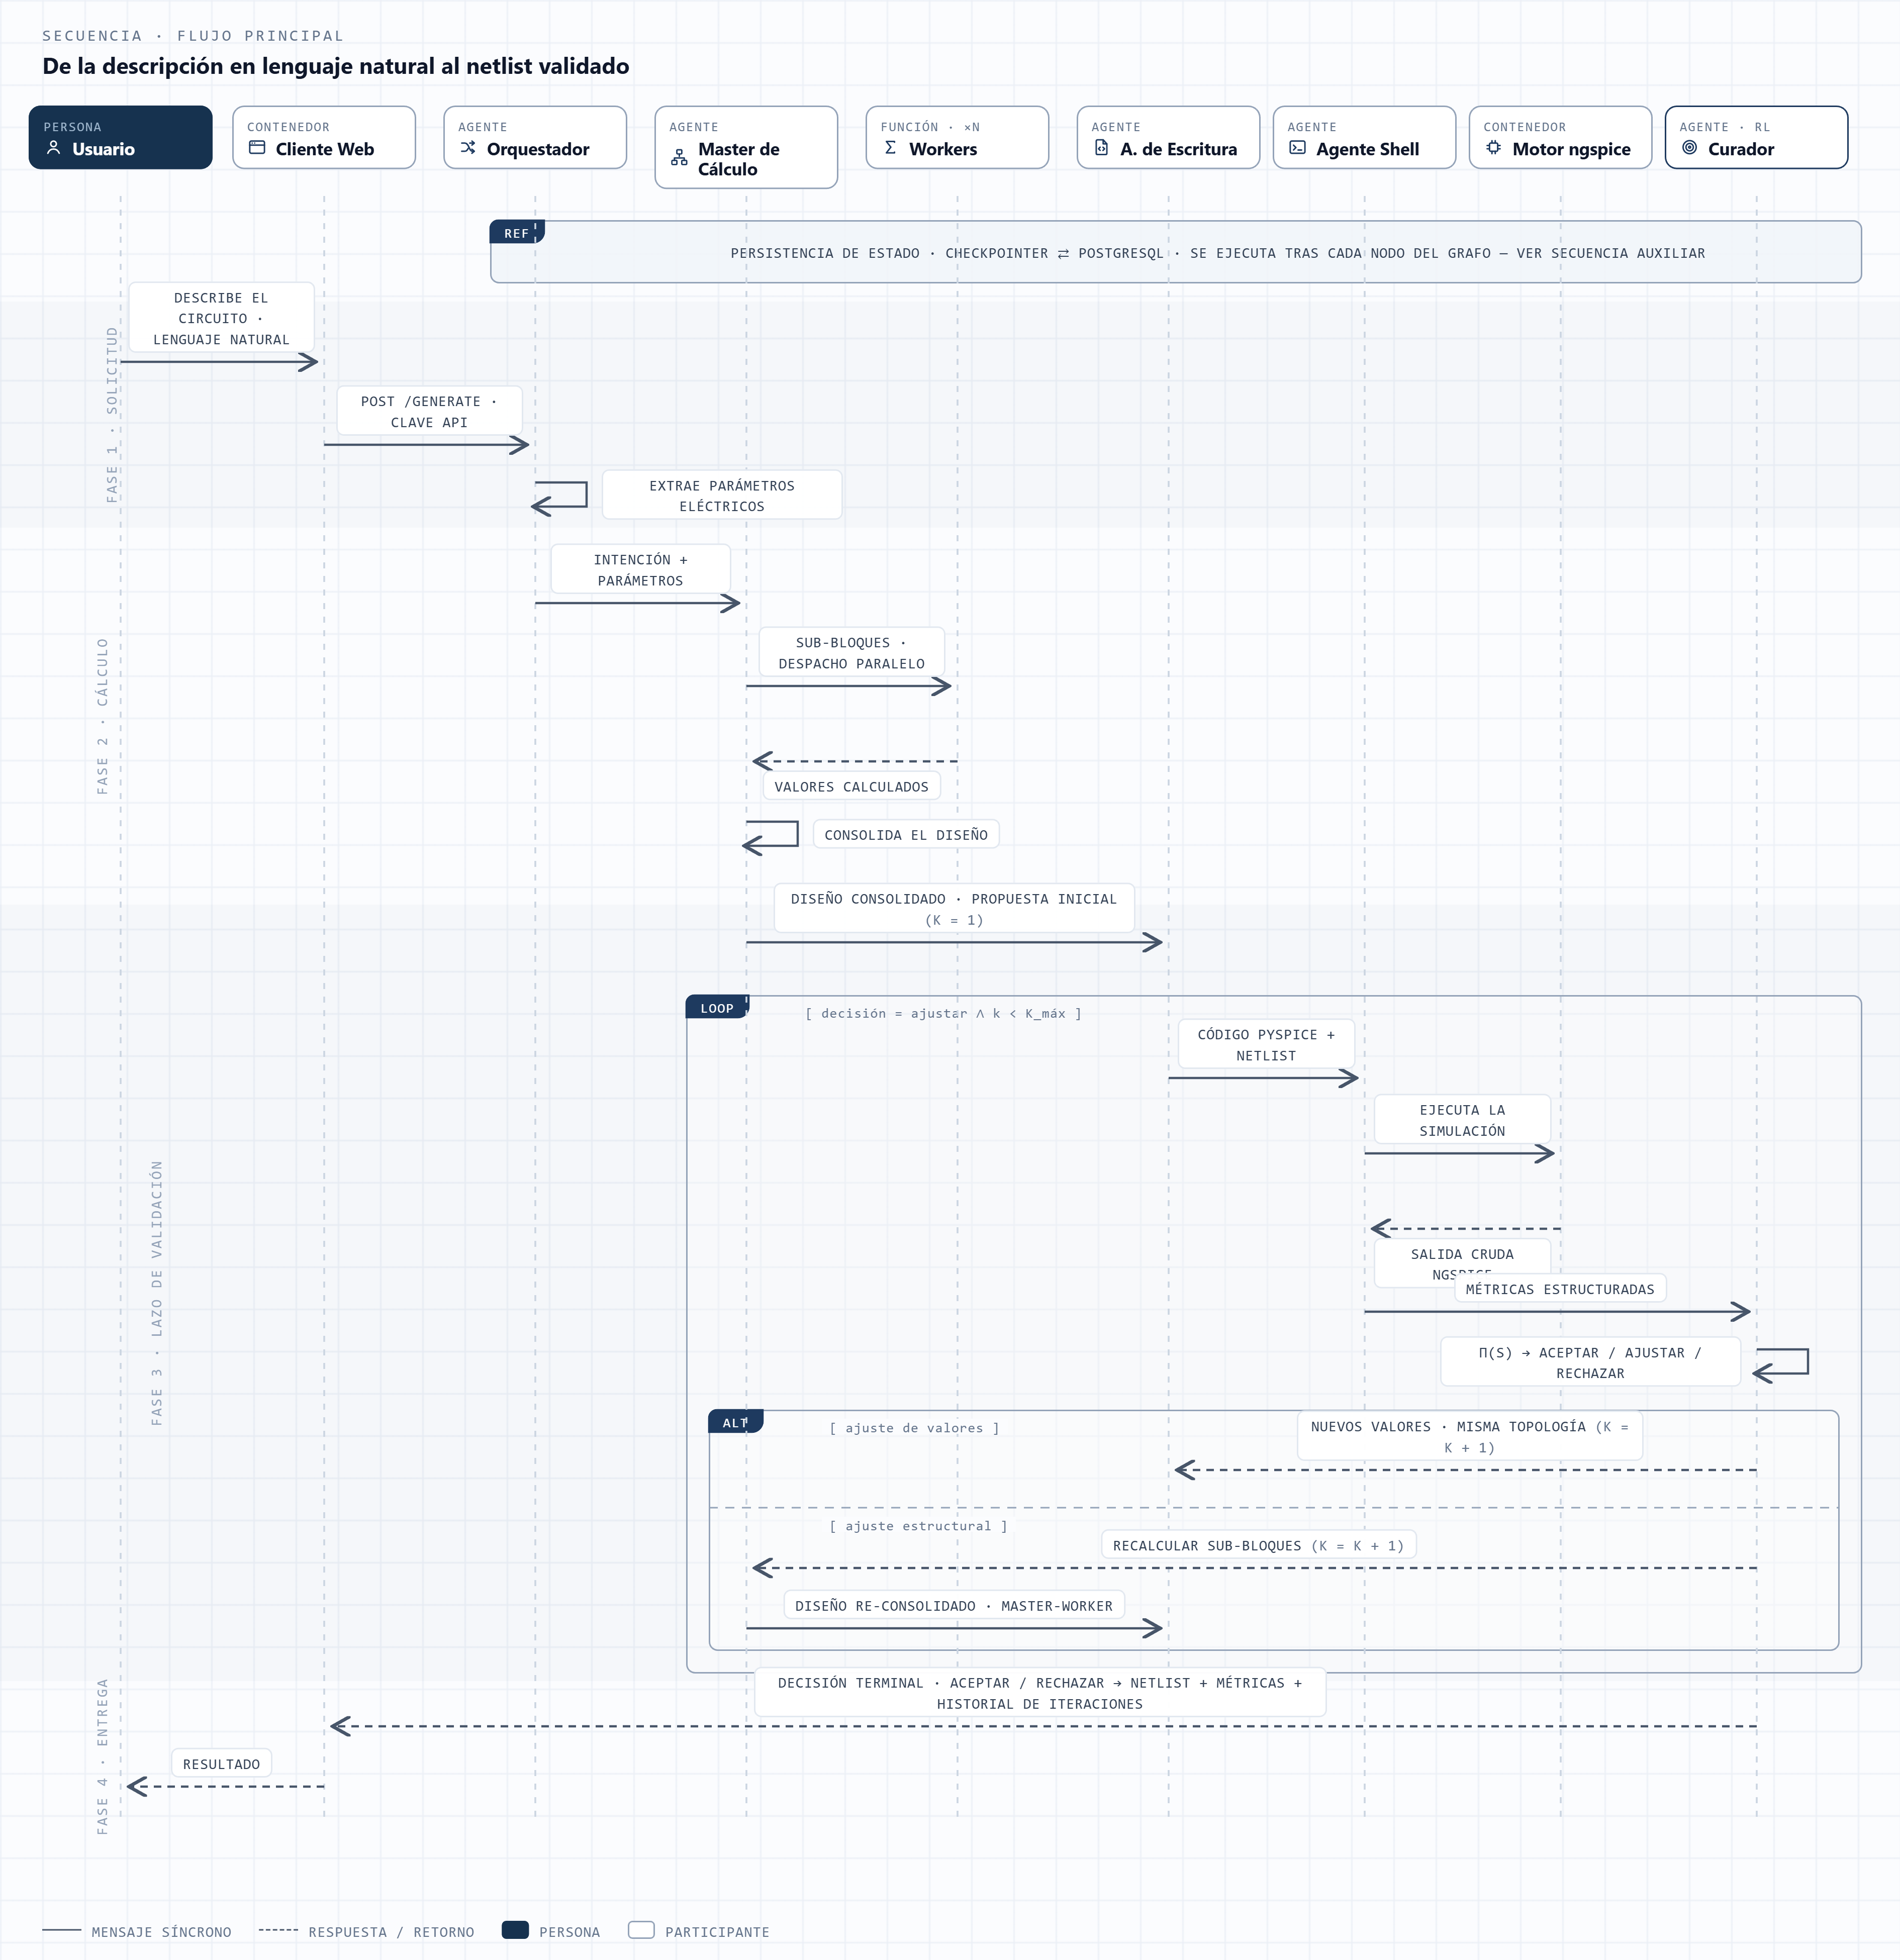
\includegraphics[width=1.3\textwidth, keepaspectratio]{../src/diagrams/secuencia_flujo_principal.png}%
    }
    \caption{Diagrama de secuencia del flujo de generación.}
    \label{fig:secuencia-generacion}
\end{figure}

\section{Calidad de la solución}
\label{sec:prop-calidad}

La calidad de la solución se entiende aquí como el grado en que el sistema satisface las necesidades para las que se diseña, evaluado sobre características observables y no sobre el juicio del diseñador. El modelo de calidad del producto de la norma ISO/IEC 25010 organiza esas características y ofrece un vocabulario común para nombrarlas \cite{iso_25010}. Se adopta el modelo de calidad del producto ---y no el de calidad en uso, centrado en la experiencia del usuario final--- porque el sistema se evalúa como un artefacto técnico operado mediante una interfaz de programación. De las características que define la norma, el diseño atiende de forma directa cinco: idoneidad funcional, fiabilidad, eficiencia de desempeño, mantenibilidad y seguridad. A ellas se suma la trazabilidad de la generación, que el SRS recoge como requisito no funcional. Cada atributo se apoya en una decisión de diseño ya expuesta y su comprobación se registra como criterio de aceptación o como requisito no funcional, cuya medición corresponde al capítulo de pruebas.

La idoneidad funcional expresa si el sistema hace lo que debe: generar, a partir de una descripción en lenguaje natural, un circuito analógico CA/CD cuyos parámetros se acercan a las metas. Esta característica es la razón de ser del sistema y se concreta en métricas que la hacen medible ---la tasa de resolución y el error porcentual absoluto medio---, contrastadas además frente a una línea base \textit{best-of-N}. El lazo de ajuste guiado por el curador es el mecanismo que la persigue: itera hasta acercar las métricas a las metas o hasta agotar el número de iteraciones.

La fiabilidad se refiere a que el sistema se comporte de forma estable ante las condiciones esperadas y ante el fallo. El diseño la atiende por tres vías. El lazo de ajuste está acotado por un número máximo de iteraciones, lo que impide que el proceso se prolongue de forma indefinida ante un circuito que no converge. El curador dispone de una decisión determinista por reglas como respaldo de su política, de modo que el sistema produce siempre una decisión aunque la política aprendida no resulte aplicable. Y el \textit{checkpointer} aporta recuperabilidad: al persistir el estado de la generación tras cada paso, una ejecución interrumpida puede retomarse desde el último punto guardado en lugar de reiniciarse, propiedad que el SRS recoge como tolerancia a fallos (RNF-03.2). La convergencia de la simulación se registra como una métrica y forma parte del estado que el curador evalúa, lo que evita que un netlist no convergente se acepte como válido.

La eficiencia de desempeño atañe al tiempo y a los recursos que el sistema consume para producir un resultado. El diseño la aborda mediante el cálculo concurrente de los sub-bloques independientes, que reduce la latencia frente a un cálculo secuencial, y mediante un límite de tiempo para el ciclo completo. El carácter sin estado del subsistema servidor habilita además su réplica detrás de un balanceador de cargas, lo que permite atender más solicitudes en paralelo sin rediseñar el sistema; esta capacidad de crecer mediante réplicas es lo que el SRS registra como escalabilidad y que el modelo de la norma sitúa dentro de la eficiencia de desempeño.

La mantenibilidad se fundamentó ya entre las premisas de diseño (sección~\ref{subsec:prop-premisas-disenio}): la modularidad de los agentes materializa la alta cohesión y el bajo acoplamiento, y la configuración externa de los pesos, los factores y los umbrales del curador permite ajustar el comportamiento del sistema sin tocar el código. Se retoma aquí para situarla dentro del modelo de calidad, no para repetir su justificación.

A la mantenibilidad se vincula la trazabilidad de la generación. El sistema conserva el historial de iteraciones y la recompensa que el curador calcula en cada ciclo, de modo que el camino que llevó a un netlist queda registrado y es posible reconstruirlo. En términos del modelo de la norma, esta propiedad se aproxima a la analizabilidad, una faceta de la mantenibilidad, pues facilita diagnosticar el comportamiento del sistema tras una ejecución. El mismo registro constituye la traza en la que se apoya el control de seguridad descrito en la sección~\ref{sec:prop-seguridad}, lo que enlaza la calidad y la seguridad sobre un único mecanismo.

La seguridad es, en el modelo ISO/IEC 25010, una característica de calidad más. Por su peso en un sistema que gestiona credenciales y claves de acceso, se trata de forma separada en la sección siguiente.

La correspondencia entre cada característica, la decisión de diseño que la atiende y el lugar donde se registra o se mide se resume a continuación.

\begin{table}[H]
\centering
\small
\caption{Correspondencia entre atributos de calidad, decisiones de diseño y evidencia de evaluación.}
\label{tab:calidad-solucion}
\vspace{0.3cm}
\renewcommand{\arraystretch}{1.35}
\rowcolors{2}{white}{rowgray}
\begin{tabularx}{\textwidth}{p{3.1cm} >{\raggedright\arraybackslash}X >{\raggedright\arraybackslash}X}
\toprule
\rowcolor{guinda}
\textcolor{white}{\textbf{Característica}} &
\textcolor{white}{\textbf{Decisión de diseño que la atiende}} &
\textcolor{white}{\textbf{Dónde se registra o mide}} \\
\midrule
Idoneidad funcional & Lazo de ajuste guiado por el curador & Tasa de resolución y MAPE; comparación con \textit{best-of-N} \\
Fiabilidad & Límite de iteraciones; respaldo determinista del curador; recuperabilidad por \textit{checkpointer}; registro de convergencia & CA-04, CA-05; RNF-03.2 \\
Eficiencia de desempeño & Cálculo concurrente; límite de tiempo; servidor sin estado replicable & RNF-01.1, RNF-01.2; CA-05, CA-06 \\
Mantenibilidad & Modularidad de los agentes; configuración externa & RNF-04.1 \\
Trazabilidad (analizabilidad) & Registro del historial de iteraciones y de la recompensa & CA-03; RNF de trazabilidad \\
Seguridad & Controles descritos en la sección~\ref{sec:prop-seguridad} & RF-06, RIMP-11 \\
\bottomrule
\end{tabularx}
\end{table}

Conviene precisar el alcance de esta evaluación de calidad. La idoneidad funcional, la fiabilidad y la eficiencia de desempeño se contrastan contra umbrales numéricos en el capítulo de pruebas. La mantenibilidad, la trazabilidad y la seguridad, en cambio, se evidencian de forma estructural ---por las propiedades del diseño y por la revisión del código y del repositorio--- y no mediante una métrica cuantitativa, lo que constituye un límite reconocido de la evaluación. Quedan fuera del foco de calidad de esta versión la usabilidad ---el sistema se opera mediante una interfaz de programación, no mediante una interfaz gráfica para usuarios finales--- y la portabilidad más allá del despliegue reproducible en contenedores.

\section{Seguridad de la solución}
\label{sec:prop-seguridad}

La seguridad del sistema se aborda en proporción a su naturaleza de prototipo académico: el objetivo no es una auditoría completa, sino controles razonables sobre los activos que el sistema maneja. Esos activos son las credenciales de los usuarios, las API keys con las que se autentican las solicitudes, los secretos del propio sistema ---la clave de la API del LLM, las credenciales de la base de datos y los secretos de Better Auth---, las descripciones y netlists de cada usuario y la integridad del estado que el servidor persiste durante la generación. El análisis se ordena con los tres principios clásicos de la seguridad informática: confidencialidad, integridad y disponibilidad \cite{stallings2018computer}.

Bajo confidencialidad se agrupan los secretos y las credenciales, que no deben quedar expuestos. A esta categoría pertenece también la descripción del circuito que el usuario envía, que el sistema transmite a un proveedor de LLM externo para su procesamiento; la confidencialidad de esos datos depende en parte de ese proveedor, dependencia que se reconoce como límite al final de la sección. La integridad se refiere a que el estado de una generación y el netlist resultante no se alteren de forma indebida entre iteraciones. La disponibilidad ---que el servicio responda a las solicitudes legítimas--- se apoya en el diseño sin estado del servidor, que admite réplicas y reduce el impacto de la caída de una instancia.

El diseño incorpora un conjunto de controles proporcionados a esos activos. La autenticación de los usuarios se delega en Better Auth \cite{betterauth}, que concentra el registro, el inicio de sesión y la gestión de sesiones en un componente especializado en lugar de implementarlos desde cero. La autorización de las solicitudes al servidor se realiza mediante API keys que el usuario emite y puede revocar, de modo que cada solicitud que llega al servidor viaja autenticada. Las API keys y los circuitos de cada usuario quedan acotados a su espacio de trabajo, por lo que la autorización no se limita a comprobar que una solicitud esté autenticada, sino a que cada usuario acceda solo a sus propios recursos. La separación entre subsistema cliente y subsistema servidor actúa como frontera de confianza: el servidor no expone la lógica de diseño a solicitudes no autenticadas y el cliente no ejecuta esa lógica. Los secretos del sistema se leen de variables de entorno y no se escriben en el código ni se versionan en el repositorio, control que el SRS recoge como requisito de manejo de secretos (RIMP-11).

Un riesgo propio de un sistema que recibe lenguaje natural y lo entrega a agentes basados en LLM es que la entrada del usuario contenga instrucciones que desvíen el comportamiento de los agentes. Para acotarlo, la descripción se valida y se restringe a los parámetros eléctricos que el orquestador necesita antes de incorporarla al proceso, y la salida del modelo se exige en un formato estructurado, lo que reduce el margen para respuestas fuera de lo previsto.

Un control específico de este sistema atiende la ejecución de artefactos producidos por el modelo. El agente de escritura genera código PySpice y un netlist, y el agente de shell los ejecuta para obtener las métricas; ejecutar código generado por un LLM es una superficie que conviene contener. El diseño la acota al ejecutar esos artefactos dentro del entorno contenedorizado del servidor, cuyo despliegue reproducible recoge el SRS (RIMP-10), de modo que la ejecución queda aislada del entorno anfitrión. El endurecimiento de ese aislamiento más allá de la contención por contenedor queda fuera del alcance de esta versión. El registro de la actividad ---entre otros, la recompensa que el curador calcula en cada iteración--- deja una traza que permite revisar el comportamiento del sistema tras una ejecución.

Los controles anteriores se corresponden con varias de las categorías de riesgo que recopila el proyecto OWASP en su lista de los diez riesgos más críticos para aplicaciones web \cite{owasp_top10}. El control de acceso por API key y el aislamiento entre espacios de trabajo atienden el riesgo de control de acceso roto; la delegación en Better Auth, el de fallos de identificación y autenticación; el manejo de secretos fuera del repositorio, el de configuración de seguridad deficiente y exposición de datos sensibles; la validación de la entrada, el de inyección; y la contención de la ejecución de artefactos generados, el de fallos de integridad del software y de los datos. La lista de OWASP se emplea como catálogo de referencia para situar los controles, no como una verificación exhaustiva de conformidad.

El alcance de seguridad de esta versión tiene límites explícitos. La comunicación entre el usuario y el sistema se realiza sobre HTTPS, pero el diseño no incorpora cifrado de los datos en reposo más allá del que provea la base de datos, ni monitoreo de seguridad especializado, ni pruebas de penetración formales, ni un modelado de amenazas exhaustivo. A ello se añaden dos límites particulares: el sistema no aplica un control de tasa sobre las solicitudes, por lo que el uso intensivo de un usuario autenticado puede consumir recursos de cómputo y llamadas al LLM sin freno; y la confidencialidad de los datos enviados al proveedor de LLM externo escapa al control directo del sistema. Todos ellos exceden el alcance de un prototipo de tesina y se señalan para delimitar con honestidad qué protege el sistema y qué no.

\section{Criterios de aceptación de la propuesta}
\label{sec:prop-criterios}

La propuesta de solución se considerará satisfactoria si el sistema construido cumple un conjunto de criterios de aceptación objetivos y comprobables de forma independiente. Estos criterios están enunciados en el SRS junto con su procedimiento de verificación, lo que permite contrastarlos con mediciones reales en lugar de con el juicio del diseñador. No se evalúan en este capítulo —su comprobación empírica corresponde al capítulo de experimentos y resultados— pero se enuncian aquí como cierre del diseño, para dejar explícito qué deberá medirse y bajo qué condición se dará por cumplido.

Entre los criterios relevantes figuran: que el sistema acepte una descripción en lenguaje natural y extraiga de ella correctamente los parámetros eléctricos; que ejecute sub-bloques independientes en paralelo; que el lazo de ajuste itere hasta cumplir la meta o alcanzar el máximo de iteraciones; que produzca un netlist simulado en ngspice; y que la salida sea repetible con la temperatura del LLM fijada, para permitir la comparación de resultados durante la evaluación.

\section{Síntesis del diseño}
\label{sec:prop-sintesis}

La propuesta de solución descrita en este capítulo da forma concreta a la brecha identificada en el estado del arte: un sistema que genera y valida circuitos analógicos CA/CD a nivel de componentes comerciales, con la simulación SPICE incorporada dentro del lazo de diseño. El diseño se articula en tres planos que se sostienen entre sí. La descomposición funcional y los casos de uso (sección~\ref{sec:prop-funcional}) establecen qué hace el sistema y quién interactúa con él. El modelo C4 en sus tres niveles (sección~\ref{sec:prop-c4}) establece cómo se estructura: la separación en subsistema cliente y subsistema servidor, y la organización del servidor como un ecosistema de agentes modulares —Orquestador, Cálculo, Curador, Shell y Escritura— coordinados sobre un grafo con estado y persistencia. El diagrama de secuencia (sección~\ref{sec:prop-dinamico}) establece cómo se comportan esos elementos en el tiempo, integrando el lazo de ajuste iterativo que distingue a la propuesta.

Los criterios de aceptación enunciados en (sección~\ref{sec:prop-criterios}) fijan la condición que el sistema construido deberá cumplir. Su comprobación —la medición del comportamiento del sistema frente a esos criterios sobre un conjunto de circuitos de prueba— constituye la evaluación del sistema y se desarrolla en el capítulo siguiente, que toma este diseño como objeto de medida.


  % CAPÍTULO 5: PRUEBAS Y ANÁLISIS DE RESULTADOS
  \chapter{Pruebas y Análisis de Resultados}
  \input{sections/pruebas}

  % CAPÍTULO 6: CONCLUSIONES Y TRABAJO FUTURO
  \chapter{Conclusiones y Trabajo Futuro}
  \input{sections/conclusiones}

  % ---------------------------------------------------------------------
  % BIBLIOGRAFÍA
  % ---------------------------------------------------------------------
  \clearpage
  \printbibliography[heading=bibintoc,title={Referencias}]

  % ---------------------------------------------------------------------
  % APÉNDICES
  % ---------------------------------------------------------------------
  \appendix
  % Apéndice A: Diagramas de casos de uso complementarios
\chapter{Diagramas de casos de uso}
\label{apend:casos-uso}

Los siguientes diagramas complementan el modelo de casos de uso presentado en la sección~\ref{subsec:prop-casos-uso}. Cada uno detalla un subconjunto de interacciones del sistema.

\begin{figure}[H]
    \centering
    \makebox[\textwidth][c]{%
        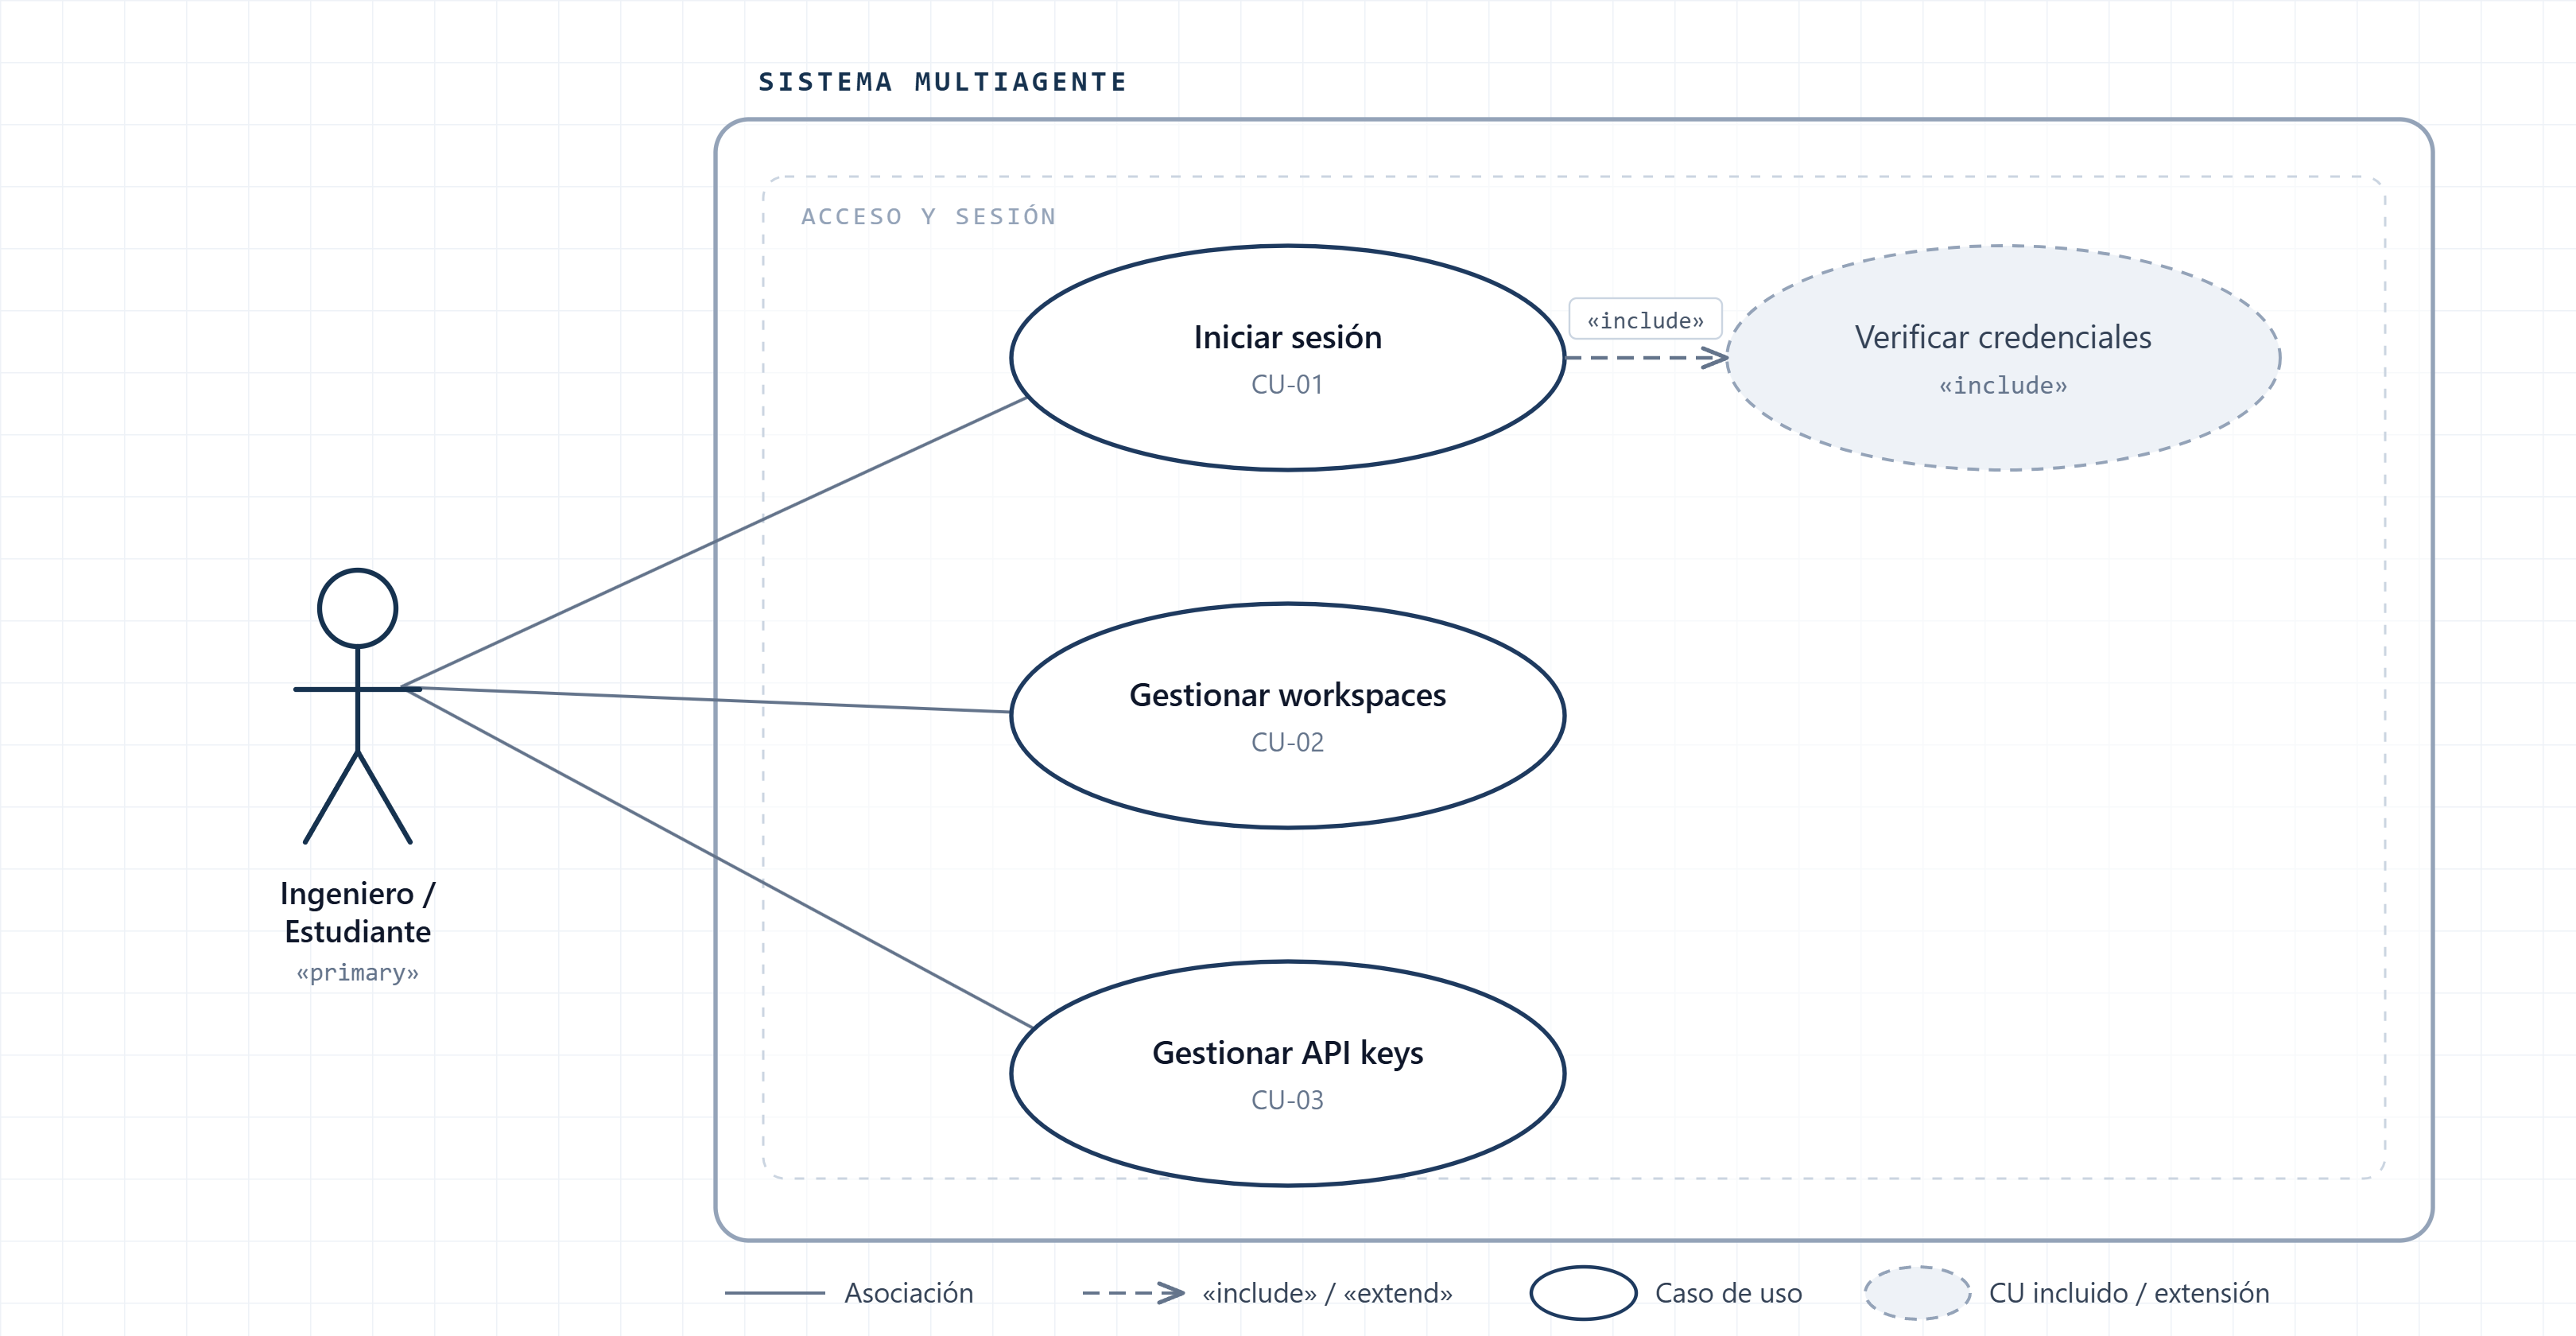
\includegraphics[width=1\textwidth, keepaspectratio]{../src/diagrams/casos_uso_acceso.png}%
    }
    \caption{Diagrama de casos de uso: acceso y gestión de sesiones.}
    \label{fig:casos-uso-acceso}
\end{figure}

\begin{figure}[H]
    \centering
    \makebox[\textwidth][c]{%
        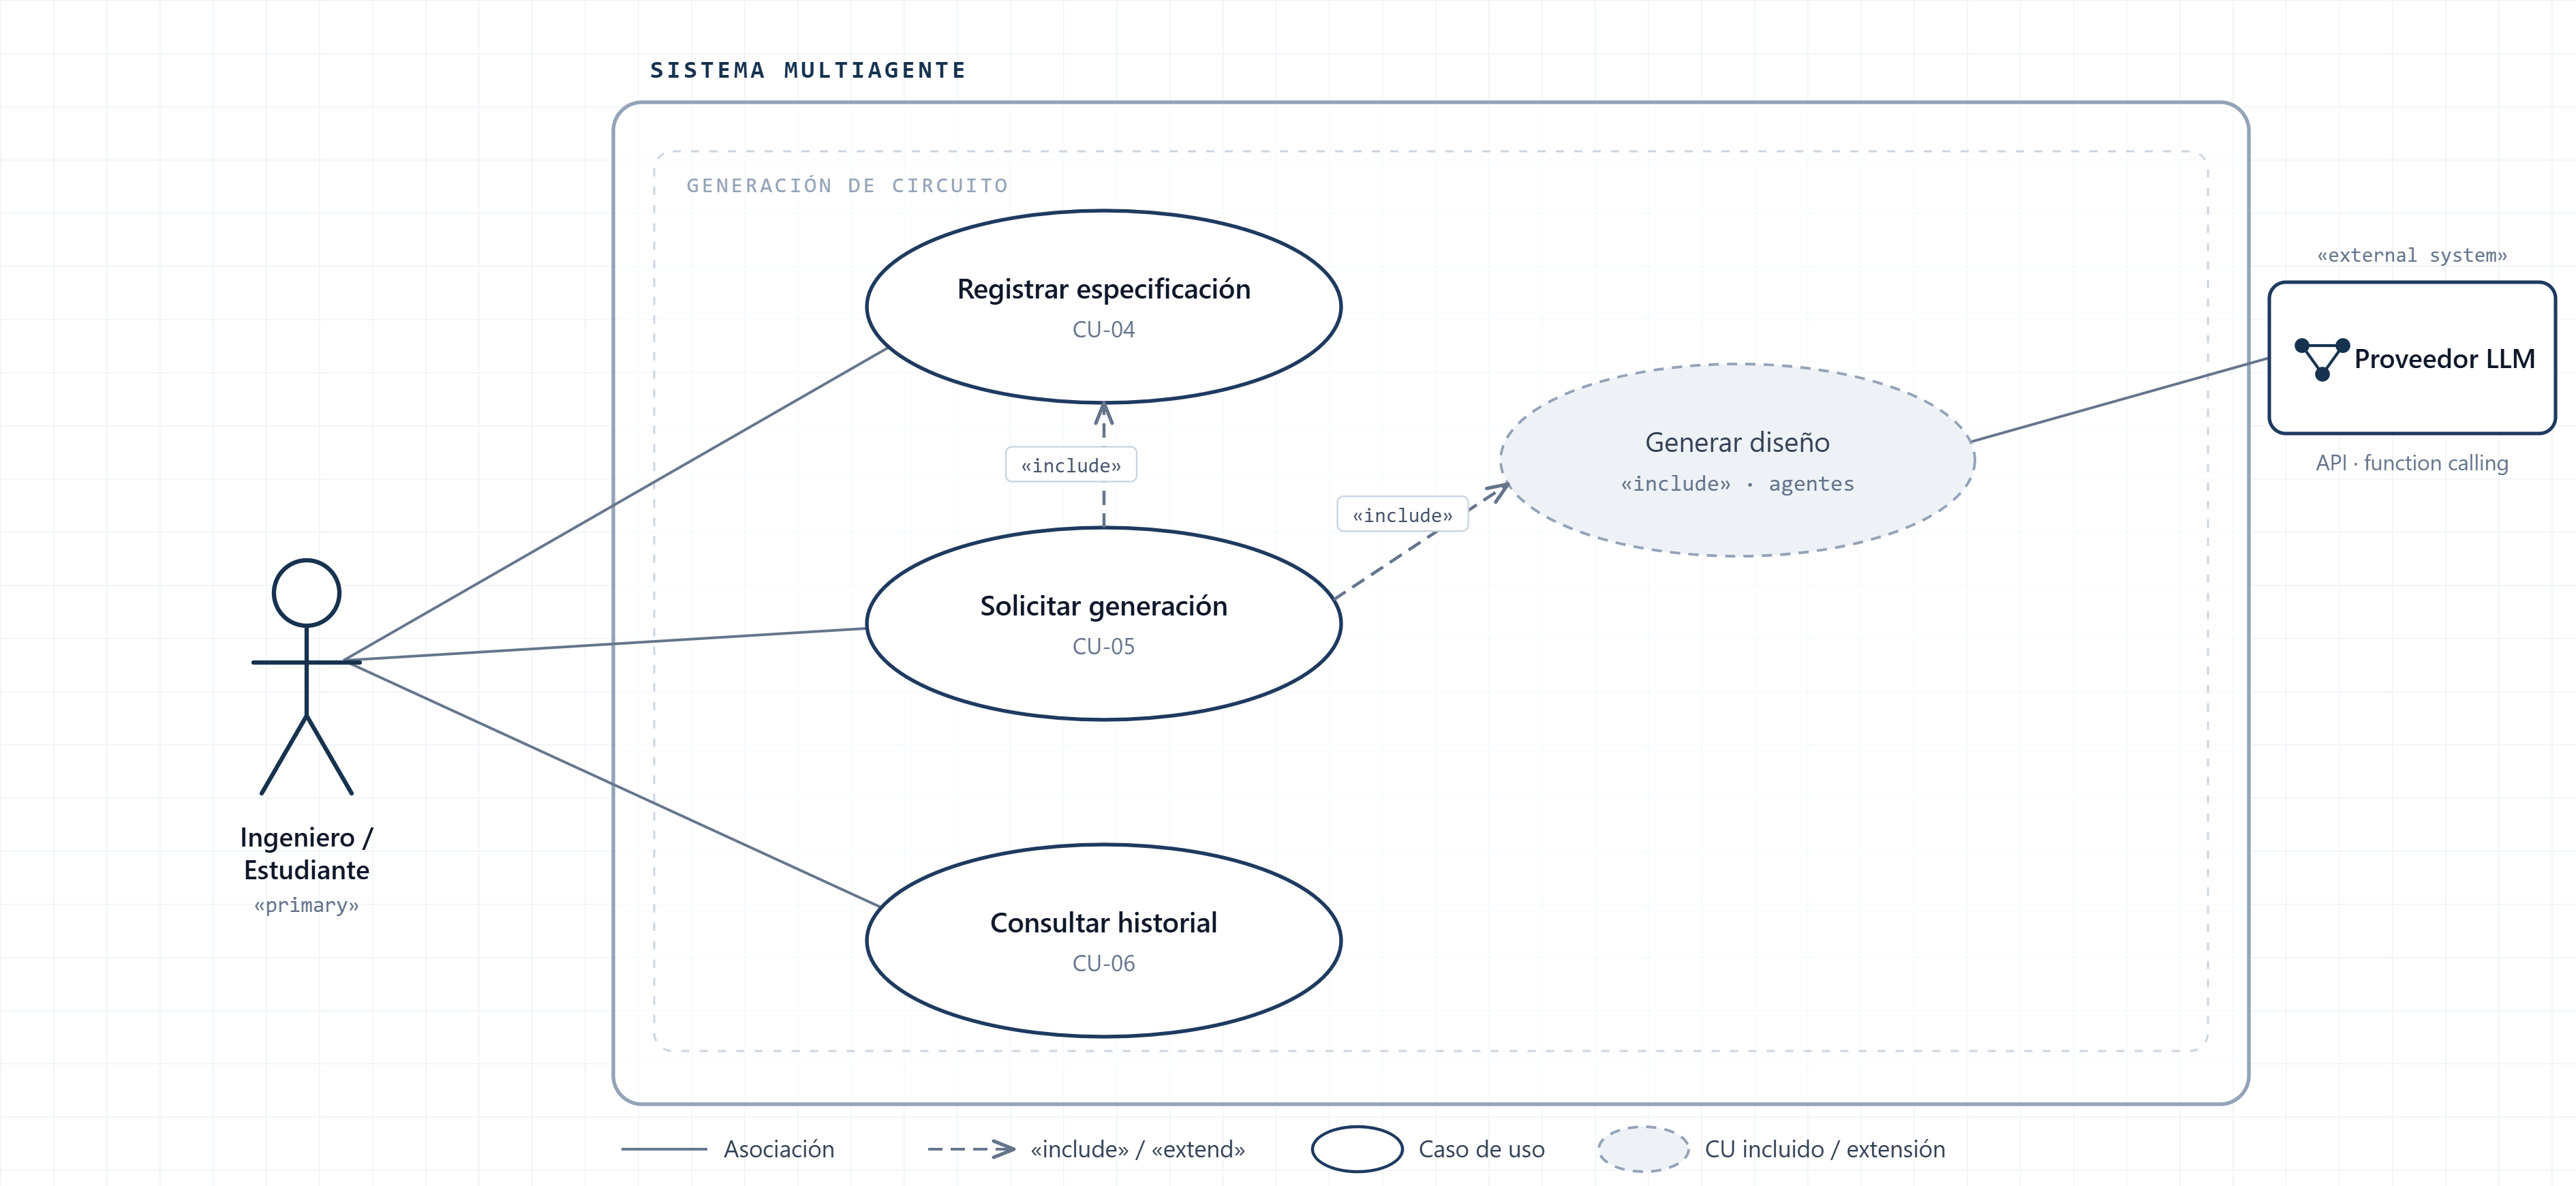
\includegraphics[width=1\textwidth, keepaspectratio]{../src/diagrams/casos_uso_generacion.png}%
    }
    \caption{Diagrama de casos de uso: generación de circuito.}
    \label{fig:casos-uso-generacion}
\end{figure}

\begin{figure}[H]
    \centering
    \makebox[\textwidth][c]{%
        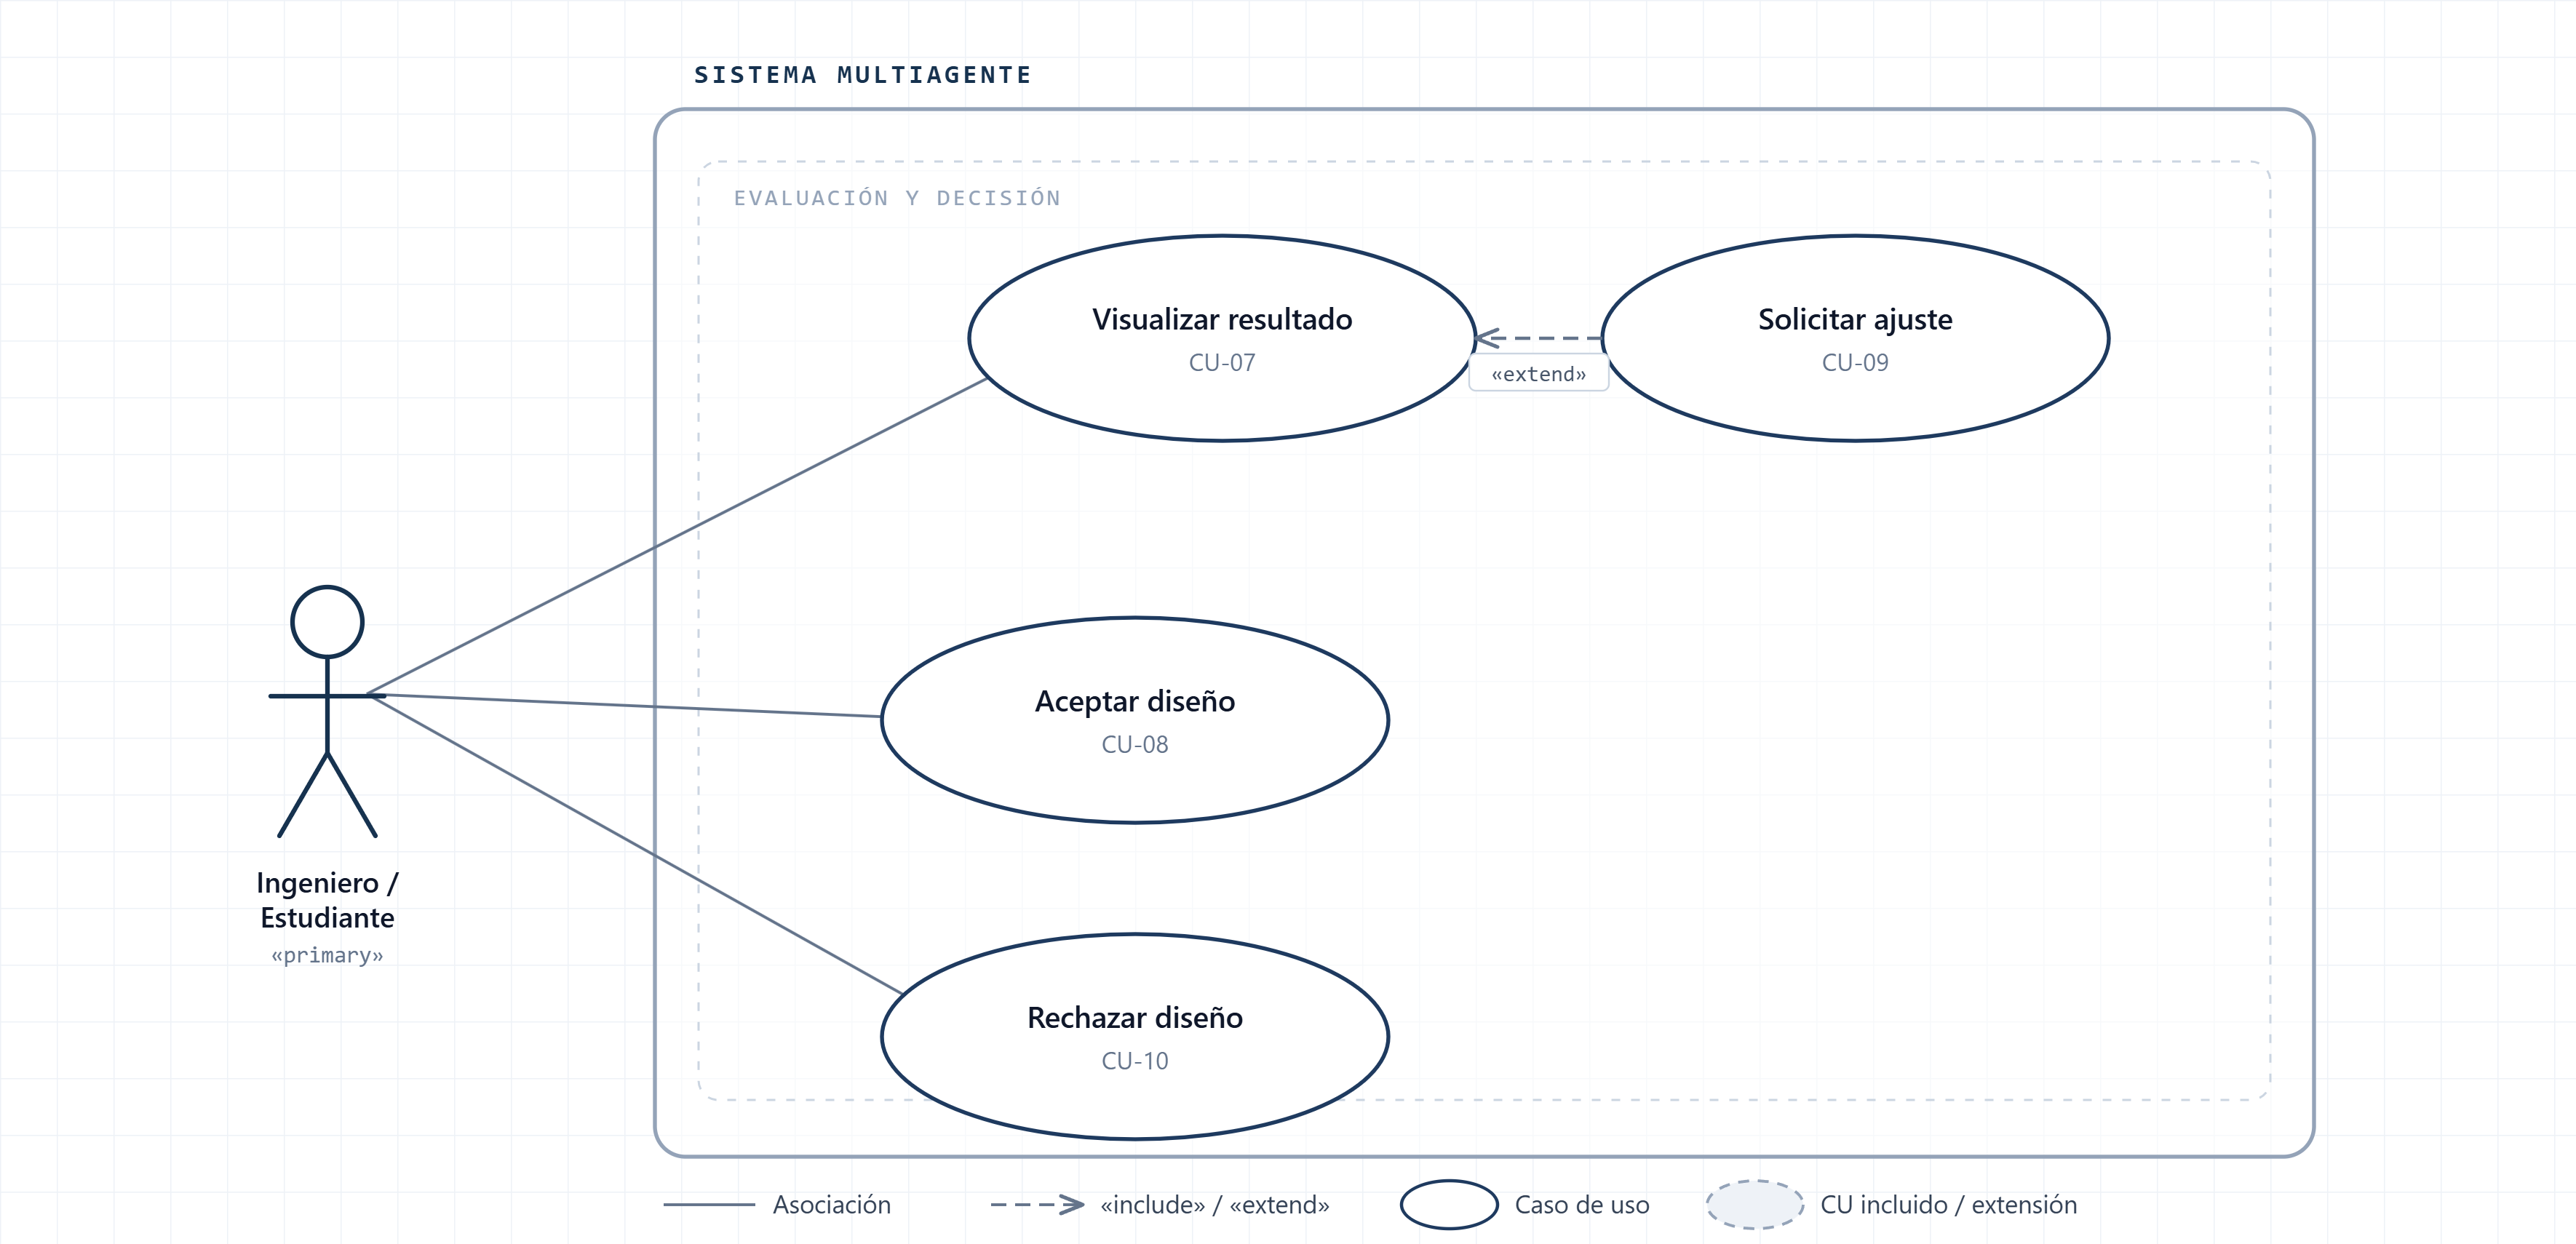
\includegraphics[width=1\textwidth, keepaspectratio]{../src/diagrams/casos_uso_decision.png}%
    }
    \caption{Diagrama de casos de uso: decisión del agente curador.}
    \label{fig:casos-uso-decision}
\end{figure}


\end{document}
